\documentclass[12pt,a4paper,openright,twoside]{book}
\usepackage[utf8]{inputenc}
\usepackage{float}
\usepackage{disi-thesis}
\usepackage{code-lstlistings}
\usepackage{notes}
\usepackage{shortcuts}
\usepackage{acronym}

% Pacchetti per le tabelle avanzate
\usepackage{tabularx}  % Tabelle a larghezza fissa con colonne adattabili (X)
\usepackage{booktabs}  % Linee professionali (\toprule, \midrule, \bottomrule)
\usepackage{float}     % Posizionamento preciso delle tabelle ([H])

\school{\unibo}
\programme{Corso di Laurea in Ingegneria e Scienze Informatiche}
\title{Generazione automatica di dataset text-to-SPARQL per fine-tuning di LLM
su knowledge graph clinico-oncologico}
\author{Matteo Tonelli}
\date{\today}
\subject{Programmazione}
\supervisor{Prof.ssa Antonella Carbonaro}
\session{II}
\academicyear{2025-2026}

\acrodef{KG}{Knowledge Graph}
\acrodef{LLM}{Large Language Model}
\acrodef{RDF}{Resource Description Framework}
\acrodef{LoRA}{Low-Rank Adaptation}
\acrodef{QLoRA}{Quantized Low-Rank Adaptation}
\acrodef{ECOG}{Eastern Cooperative Oncology Group}
\acrodef{TNM}{Tumor, Node, Metastasis}
\acrodef{HPC}{High Performance Computing}
\acrodef{GPU}{Graphics Processing Unit}
\acrodef{API}{Application Programming Interface}
\acrodef{HL7}{Health Level Seven}
\acrodef{FHIR}{Fast Healthcare Interoperability Resources}
\acrodef{IRI}{Internationalized Resource Identifier}

\mainlinespacing{1.241} 

\begin{document}

\frontmatter\frontispiece

\begin{abstract}
    Il lavoro proposto si colloca nel progetto Cancer Virtual Lab (CVL), il
    quale raccoglie i dati clinici oncologici dell'IRCCS IRST "Dino Amadori" in
    un Knowledge Graph interrogabile tramite SPARQL\footnote{W3C SPARQL 1.1
        Query Language Recommendation:
        \url{[https://www.w3.org/TR/sparql11-query/](https://www.w3.org/TR/sparql11-query/)}}.
    La natura formale di SPARQL rappresenta però una barriera per il personale
    sanitario e un'interfaccia in linguaggio naturale (Text-to-SPARQL)
    permetterebbe di abbattere tale barriera, ma richiederebbe un modello
    linguistico addestrato sull'ontologia specifica di CVL, per la quale non
    esistono dataset di addestramento pubblici.

    Questo lavoro progetta e implementa una pipeline automatizzata a due stadi
    per la generazione di un dataset Text-to-SPARQL sintetico, garantendo
    correttezza e varietà. Il primo stadio esplora lo schema del grafo e
    campiona combinazioni di vincoli sintatticamente corrette, coprendo diverse
    entità organizzate in gruppi di priorità basati sulla centralità clinica. Il
    secondo stadio applica un meccanismo di mascheramento dei valori letterali e
    un ciclo iterativo di parafrasi guidata per generare varianti in più
    registri stilistici distinti, aumentando la ricchezza linguistica senza
    alterare la semantica delle query.

    La pipeline ha prodotto in fase di testing un dataset di 14.021 esempi,
    strutturato con una rigorosa separazione per record sorgente tra gli insiemi
    di addestramento, validazione e test per evitare data leakage. Un modello
    \texttt{Gemma3:270M}, sottoposto a fine-tuning mediante LoRA su questo
    dataset, ha raggiunto un exact match del 46\% sull'insieme di test
    in-distribution, individuando il checkpoint ottimale tramite validation loss
    e superando nettamente il full fine-tuning (18\%). L'analisi degli errori
    residui ha mostrato un tasso dello 0\% di query sintatticamente non valide,
    dimostrando che il modello apprende saldamente la grammatica SPARQL. Vengono
    infine analizzati i problemi di qualità emersi nel dataset, delineando le
    relative strategie di risoluzione.
\end{abstract}


\tableofcontents
\listoffigures
\lstlistoflistings

\mainmatter

\chapter{Introduzione}
\label{chap:introduction}

Il Cancer Virtual Lab (CVL) è una piattaforma che raccoglie i dati clinici
oncologici dell'IRST "Dino Amadori" in un knowledge graph interrogabile tramite
SPARQL, il linguaggio di interrogazione standard per i dati strutturati secondo
il modello RDF (\cref{chap:background}). SPARQL è un linguaggio formale, e la
sua sintassi richiede una competenza tecnica che il personale clinico e i
ricercatori del dominio oncologico non possiedono tipicamente, creando una
barriera tra la ricchezza dei dati disponibili e la possibilità concreta di
interrogarli senza il supporto di uno specialista informatico. Un'interfaccia in
linguaggio naturale capace di tradurre una domanda posta in italiano o in
inglese nella query SPARQL corrispondente ridurrebbe questa barriera, ma
richiede un modello linguistico specificamente addestrato a questo compito: un
modello generico, per quanto capace su compiti generali, non conosce la
struttura specifica dell'ontologia di CVL, i nomi delle sue classi e proprietà,
né le convenzioni con cui le query sono tipicamente costruite in questo
contesto.

Addestrare un simile modello richiede a sua volta un dataset di addestramento
composto da coppie di domande in linguaggio naturale e query SPARQL
corrispondenti, specifiche per l'ontologia di CVL. Un dataset di questo tipo non
esiste in partenza, e costruirlo manualmente, coppia per coppia, non è una
strada praticabile alla scala necessaria per un addestramento efficace. Questo
lavoro affronta questo problema progettando e implementando una pipeline
automatica in grado di generare un simile dataset, e ne verifica l'efficacia
addestrando concretamente un modello linguistico sui dati prodotti.

La pipeline sviluppata si articola in due stadi. Il primo genera in modo
strutturato coppie di prompt e query SPARQL valide, esplorando sistematicamente
lo schema del knowledge graph e campionando combinazioni di vincoli
sintatticamente corrette. Il secondo arricchisce ciascuna coppia con più
formulazioni linguistiche alternative della stessa domanda, aumentando la
varietà stilistica del dataset senza alterarne la correttezza semantica. Il
modello linguistico risultante dal fine-tuning su questo dataset è stato infine
valutato sperimentalmente, confrontando diverse configurazioni di addestramento
e analizzando la natura degli errori residui.

\section*{Struttura della tesi}

Il \cref{chap:background} introduce il contesto tecnico necessario a seguire il
resto del lavoro: la piattaforma CVL, i concetti di knowledge graph, RDF e
SPARQL, i lavori correlati sulla generazione di dataset text-to-SPARQL, e le
tecniche di fine-tuning di modelli linguistici impiegate più avanti. Il
\cref{chap:analisi} definisce gli obiettivi, i vincoli e i requisiti del
sistema. Il \cref{chap:progettazione} descrive le decisioni progettuali alla
base sia del generatore sia dello stadio di augmentation. Il
\cref{chap:implementation} ne documenta l'implementazione concreta. Il
\cref{chap:evaluation} riporta i risultati sperimentali, sia sul dataset
prodotto sia sul modello linguistico addestrato a partire da esso. Il
\cref{chap:conclusion} chiude il lavoro con una sintesi dei risultati ottenuti e
le direzioni di sviluppo future.

\chapter{Background}
\label{chap:background}

Questo capitolo fornisce il quadro teorico, metodologico e tecnologico
necessario a comprendere il contesto applicativo e le decisioni progettuali alla
base dell'intero lavoro di tesi. La generazione automatica di dataset sintetici
per la traduzione da linguaggio naturale a linguaggi formali di interrogazione
(\textit{Text-to-SPARQL}) si colloca infatti all'intersezione tra diverse
discipline informatiche: l'ingegneria del Web Semantico, la modellazione di dati
clinici e il \textit{Natural Language Processing} (NLP) applicato ai modelli
linguistici di grandi dimensioni (\textit{Large Language Model}, LLM).

Per fornire una visione più strutturata, il capitolo è organizzato in cinque
sezioni interconnesse:

\begin{itemize}
    \item \textbf{Cancer Virtual Lab (\cref{sec:bg-cvl}):} descrive la
          piattaforma del Cancer Virtual Lab (CVL), illustrando le sfide legate
          alla frammentazione dei dati oncologici, l'adozione dello standard
          internazionale HL7 FHIR e le motivazioni cliniche che guidano la
          realizzazione di un'interfaccia di interrogazione in linguaggio
          naturale.

    \item \textbf{Knowledge Graph, RDF e Strumenti SPARQL
              (\cref{sec:bg-kg-sparql}):} introduce le nozioni fondamentali sui
          Knowledge Graph e sul modello di rappresentazione a triple RDF
          (\textit{Resource Description Framework}). Viene inoltre
          approfondito il linguaggio di interrogazione SPARQL, insieme al
          ruolo degli strumenti software locali (in particolare la libreria
          Python
          \texttt{rdflib})\footnote{\url{[https://rdflib.readthedocs.io/en/stable/](https://rdflib.readthedocs.io/en/stable/)}}
          utilizzati per la validazione sintattica deterministica delle
          query.

    \item \textbf{Architettura Software e Pattern
              (\cref{sec:bg-software-tools}):} analizza le scelte tecnologiche e
          i pattern di progettazione software adottati nell'ingegneria del
          sistema, tra cui l'architettura a \textit{Mixin} per la
          composizione modulare delle responsabilità e il framework
          \texttt{Streamlit}\footnote{\url{[https://streamlit.io/](https://streamlit.io/)}}
          per la prototipazione di interfacce interattive di monitoraggio e
          controllo.

    \item \textbf{Lavori Correlati e Benchmark di Text-to-SPARQL
              (\cref{sec:bg-related-work}):} presenta una rassegna dello stato
          dell'arte sui dataset di riferimento per il compito di traduzione
          Text-to-SPARQL, evidenziando le limitazioni dei benchmark generali
          (come LC-QuAD) quando applicati a domini specialistici e
          analizzando le criticità legate all'uso diretto di modelli
          generativi senza meccanismi di contenimento delle allucinazioni.

    \item \textbf{Fine-Tuning di Modelli Linguistici nel Dominio Clinico
              (\cref{sec:bg-finetuning}):} approfondisce le tecniche di
          adattamento supervisionato (SFT), ponendo a confronto il
          \textit{Full Fine-Tuning} con le strategie di addestramento
          efficiente \textit{Parameter-Efficient Fine-Tuning} (PEFT) come
          LoRA e QLoRA. La sezione motiva inoltre la scelta di modelli
          ultra-compatti per l'esecuzione locale su dati sensibili e
          descrive l'adozione del mascheramento della loss sui token di
          input (\textit{Completion-Only Data Collator}).
\end{itemize}

\section{Cancer Virtual Lab}
\label{sec:bg-cvl}

Il lavoro descritto in questa tesi si inserisce direttamente nel contesto
applicativo e tecnologico del progetto \textit{Cancer Virtual Lab} (CVL)
\cite{cvl2025platform}, una piattaforma avanzata di \textit{AI Semantica}
progettata per supportare la ricerca oncologica e la pratica clinica guidata dai
dati. Il progetto è frutto di una collaborazione multidisciplinare tra enti di
ricerca clinica e tecnologica, tra cui l'IRCCS Istituto Romagnolo per lo Studio
dei Tumori (IRST) "Dino Amadori" di Meldola e l'Università di Bologna.

\subsection{La Sfida della Frammentazione dei Dati Clinici}
Nel contesto della pratica oncologica reale, le informazioni cliniche e
diagnostiche dei pazienti risultano intrinsecamente eterogenee, complesse e
frammentate. I dati sanitari si trovano tipicamente segregati all'interno di
silos informativi autonomi e non comunicanti:
\begin{itemize}
    \item \textit{Cartelle Cliniche Elettroniche (EHR):} contenenti la storia
          anamnestica, le visite oncologiche e il tracciamento dei ricoveri;
    \item \textit{Sistemi Informativi di Anatomia Patologica:} contenenti i
          referti istologici e la caratterizzazione molecolare del tumore;
    \item \textit{Registri Farmaceutici e Somministrazioni:} contenenti il
          dettaglio dei protocolli chemioterapici, immunoterapici e delle linee
          di trattamento;
    \item \textit{Laboratori di Analisi e Diagnostica per Immagini:} contenenti
          la serie storica degli esami ematochimici e le valutazioni strumentali
          di risposta lesionale.
\end{itemize}

Tale frammentazione costituisce una barriera sostanziale alla riutilizzabilità
secondaria dei dati per scopi di ricerca clinica. Attività fondamentali come
l'identificazione di coorti di pazienti con specifiche caratteristiche
molecolari, la valutazione dell'efficacia di terapie neoadiuvanti o l'analisi
dell'insorgenza di tossicità severe ed eventi avversi richiedono un processo
lungo e oneroso di estrazione e riconciliazione manuale delle informazioni.

\subsection{Standard di Interoperabilità: da HL7 FHIR a RDF}
Per superare la rigidità dei silos informativi, la piattaforma CVL adotta
un'architettura integrata di trasformazione semantica dei dati
\cite{cvl2025pipeline}. Il punto d'ingresso per la standardizzazione delle
informazioni cliniche è rappresentato dallo standard internazionale \ac{FHIR},
sviluppato dall’organizzazione HL7. FHIR definisce un insieme di modelli di dati
modulari e tipizzati, denominati \textit{Risorse} (es. \texttt{Patient},
\texttt{Condition}, \texttt{MedicationStatement}, \texttt{Observation}),
progettati per facilitare lo scambio sicuro di informazioni tra sistemi sanitari
eterogenei.

Tuttavia, mentre FHIR eccelle come formato di interscambio operativo via API
RESTful, le interrogazioni analitiche su relazioni complesse e multi-livello
traggono maggiore beneficio da modelli orientati ai grafi. Per questo motivo, la
pipeline di CVL mappa e trasforma le risorse FHIR anonimizzate in un Knowledge
Graph interoperabile basato sullo standard W3C \ac{RDF} \cite{cvl2025pipeline}.
Questo processo ha consentito la costruzione di una base di conoscenza semantica
integrata comprendente i dati clinici, diagnostici e terapeutici di oltre 35.000
pazienti afferenti all'IRST "Dino Amadori".

\subsection{L'Assistente Virtuale e la Necessità di Dataset Dedicati}
Un componente centrale nell'architettura della piattaforma CVL è lo sviluppo di
un assistente virtuale basato su \acfp{LLM}, concepito per consentire a medici,
oncologi e ricercatori di interrogare la base di conoscenza direttamente in
linguaggio naturale (italiano o inglese). L'obiettivo primario è eliminare la
barriera tecnica rappresentata dal linguaggio SPARQL: per un professionista
sanitario, infatti, la formulazione di una query formale richiede non soltanto
la padronanza di una sintassi rigida basata su grafi, ma anche la conoscenza
approfondita e mnemonica della struttura dell'ontologia, dei nomi specifici dei
predicati e dei vocabolari controllati adottati.

Per realizzare tale interfaccia, la semplice adozione di un modello linguistico
generico di grande taglia (\textit{off-the-shelf}) o l'affidamento a servizi
commerciali via API esterne risultano strategie inapplicabili, per tre ragioni
fondamentali:
\begin{enumerate}
    \item \textit{Mancanza di conoscenza ontologica specifica (\textit{Ontology
                  Gap}):} Un LLM pre-addestrato su corpora generici non conosce
          le convenzioni di modellazione interne al Cancer Virtual Lab.
          Se interpellato su un dominio specialistico, il modello tende
          ad allucinare predicati plausibili nel linguaggio comune ma
          inesistenti nel grafo RDF di produzione, generando query
          sintatticamente corrette ma semanticamente vuote o
          ineseguibili.

    \item \textit{Vincoli di riservatezza e trattamento dei dati sanitari:} Le
          normative sulla protezione dei dati in ambito medico (quali il GDPR) e
          la presenza di dati clinici sensibili impongono l'adozione di modelli
          eseguiti interamente in locale. Ciò preclude l'uso di modelli cloud
          proprietari e richiede la specializzazione di architetture locali di
          dimensioni contenute, che necessitano di un addestramento mirato per
          compensare la minore capacità parametrica generale.

    \item \textit{Rigore sintattico ed esecuzione deterministica:} A differenza
          della generazione di testo naturale, la traduzione
          \textit{Text-to-SPARQL} non ammette imprecisioni. Anche un singolo
          errore di formattazione, una parentesi non bilanciata o un
          identificativo errato rendono l'intera query ineseguibile
          dall'endpoint del triplestore.
\end{enumerate}

La specializzazione di un modello linguistico locale per questo compito
specifico richiede la tecnica del \textit{Supervised Fine-Tuning} (SFT), la
quale necessita a sua volta di un dataset di addestramento di alta qualità
composto da coppie di domande in linguaggio naturale e query SPARQL
corrispondenti.

Tuttavia, un dataset di questo tipo non esiste in partenza per l'ontologia di
CVL. La sua costruzione manuale, affidata alla scrittura congiunta di esperti di
dominio clinico e di ingegneri del Web Semantico, richiederebbe tempi
inaccettabili e non garantirebbe la copertura sistematica delle combinazioni di
vincoli possibili. La progettazione e l'implementazione di una pipeline
automatizzata in grado di sintetizzare un dataset di addestramento accurato,
vario e verificabile costituisce quindi il prerequisito fondamentale e la
motivazione primaria del presente lavoro di tesi.

\section{Knowledge Graph, RDF e Strumenti SPARQL}
\label{sec:bg-kg-sparql}

Per comprendere le scelte architetturali della piattaforma CVL e le sfide legate
alla generazione delle query, è necessario formalizzare il modello di dati
sottostante. L'organizzazione delle informazioni cliniche non si basa su tabelle
relazionali tradizionali, ma sul paradigma dei \acfp{KG} e sugli standard del
Web Semantico raccomandati dal W3C.

\subsection{Dai Dati Strutturati ai Knowledge Graph}
Un \ac{KG} è una struttura dati orientata a grafo, progettata per rappresentare
la conoscenza integrando entità, attributi e relazioni. A differenza delle basi
di dati relazionali tradizionali, dove i dati sono vincolati a schemi rigidi
suddivisi in tabelle e chiavi esterne, un Knowledge Graph esprime la conoscenza
in modo flessibile ed esplicito:
\begin{itemize}
    \item \textit{I Nodi} rappresentano le entità concrete del dominio (es. un
          specifico paziente, una diagnosi, un farmaco);
    \item \textit{Gli Archi Diretti} rappresentano le relazioni semantiche
          tipizzate che collegano un nodo all'altro (es. \texttt{ha\_diagnosi},
          \texttt{assume\_farmaco}).
\end{itemize}

Questo approccio risulta particolarmente vantaggioso in ambito oncologico, dove
la struttura dei dati è intrinsecamente complessa e soggetta a continua
evoluzione, dove nuove proprietà o relazioni possono essere introdotte nel grafo
senza dover ridefinire lo schema globale dell'intera base di dati.

\subsection{Resource Description Framework (RDF)}
Lo standard formale impiegato per concretizzare un Knowledge Graph è il
\acf{RDF}. In RDF, qualsiasi informazione o asserzione viene scomposta nella sua
unità elementare atomica chiamata \textit{tripla}:
\[
    (\text{Soggetto}, \text{Predicato}, \text{Oggetto})
\]
Ciascun elemento della tripla svolge un ruolo preciso nella rete di conoscenza:
\begin{itemize}
    \item \textit{Soggetto:} identifica l'entità principale dell'asserzione
          mediante un \ac{IRI}, un indirizzo univoco a livello globale;
    \item \textit{Predicato:} esprime la relazione specifica o la proprietà
          descritta, anch'esso identificato da un IRI ;
    \item \textit{Oggetto:} rappresenta il punto di arrivo della relazione. Può
          essere a sua volta un IRI che punta a un'altra entità del grafo (dando
          origine a una struttura di nodi interconnessi) oppure un valore
          letterale (\textit{Literal}) tipizzato (es. una stringa, un numero
          intero, una data ISO 8601 o un valore booleano).
\end{itemize}

L'insieme di tutte le triple forma il grafo RDF. Le regole formali, i vocabolari
controllati e la gerarchia di classi ammesse all'interno del grafo costituiscono
l'\textit{ontologia} del sistema, ovvero lo schema concettuale del dominio
clinico.

\subsection{SPARQL}
Per estrarre informazioni e interrogare un grafo RDF si utilizza SPARQL
(\textit{SPARQL Protocol and RDF Query Language}), il linguaggio di
interrogazione standard per i dati del Web Semantico.

A differenza di SQL, che opera eseguendo operazioni di join tra tabelle, SPARQL
funziona tramite il meccanismo del \textit{graph pattern matching}
(corrispondenza di schemi di grafo). La clausola \texttt{WHERE} di una query
SPARQL definisce un insieme di "triple con incognite" (dette \textit{triple
    pattern}), in cui alcuni elementi sono sostituiti da variabili identificate dal
prefisso \texttt{?} (es. \texttt{?patient}, \texttt{?diagnosis}). L'algoritmo di
esecuzione confronta lo schema richiesto con il grafo RDF reale, individuando
tutti i sotto-grafi che soddisfano simultaneamente le combinazioni di vincoli
specificate.

Per raffinare la ricerca, SPARQL mette a disposizione clausole espressive quali:
\begin{itemize}
    \item \texttt{FILTER}: applica vincoli logici, algebrici o temporali sui
          valori letterali (es. restringere la ricerca a pazienti nati entro un
          determinato intervallo di date);
    \item \texttt{VALUES}: limita i valori assegnabili a una variabile a un
          elenco discreto e prefissato;
    \item \texttt{OPTIONAL}: consente di estrarre attributi accessori senza
          compromettere la restituzione dei risultati principali qualora il dato
          non sia presente nel grafo per un determinato paziente.
\end{itemize}

\subsection{Validazione Sintattica Determinista con RDFLib}
Poiché le query SPARQL generate dalla pipeline sintetica dovranno servire da
target per l'addestramento di un modello di linguaggio, la presenza di errori di
sintassi comprometterebbe l'efficacia dell'apprendimento.

Per garantire la validità formale delle query senza dover sovraccaricare
l'endpoint SPARQL di produzione con continue chiamate di rete, il sistema
sfrutta la libreria Python \texttt{rdflib}. \texttt{rdflib} fornisce un parser
sintattico deterministico che analizza l'albero sintattico astratto
(\textit{AST}) della query generata in locale. Qualora la query presenti
parentesi non bilanciate, keyword errate o sintassi SPARQL 1.1 non conforme, il
parser solleva un'eccezione, consentendo alla pipeline di scartare o rigenerare
immediatamente l'esempio difettoso.

\section{Architettura Software e Pattern}
\label{sec:bg-software-tools}

La progettazione di pipeline complesse per l'elaborazione di dati e la sintesi
di corpora richiede l'adozione di modelli di programmazione e strumenti software
in grado di garantire modularità, manutenibilità e rapidità di ispezione. In
questa sezione vengono analizzati, a livello teorico e metodologico, i
principali pattern di progettazione ad oggetti e i paradigmi di prototipazione
rapida considerati nell'ambito del progetto.

\subsection{Il Pattern Architetturale Mixin}
Nello sviluppo di sistemi orientati agli oggetti, la gestione di processi
complessi multi-stadio richiede una rigorosa separazione delle responsabilità
per rispettare i principi SOLID, con particolare riferimento al principio di
singola responsabilità (\textit{Single Responsibility Principle}). Quando una
singola classe accumula funzionalità eterogenee, quali la gestione della
comunicazione di rete, il parsing dei dati, la logica di campionamento e le
operazioni di I/O su disco, la struttura del codice tende a diventare
monolitica, rigida e complessa da sottoporre a test.

Per risolvere tale criticità senza ricorrere ad architetture sproporzionatamente
articolate, la programmazione orientata agli oggetti mette a disposizione il
pattern \textit{Mixin}. Un Mixin si definisce come una classe progettata non per
rappresentare una struttura di dati autonoma, bensì per fornire un insieme
circoscritto e coerente di metodi a un'altra classe mediante l'impiego
dell'ereditarietà multipla. A differenza dell'ereditarietà classica, la quale
esprime una relazione di specializzazione fra tipi, il Mixin introduce una
relazione di estensione funzionale.

Tale approccio comporta tre proprietà fondamentali sul piano teorico. In primo
luogo, la classe Mixin non viene mai istanziata direttamente nel flusso di
esecuzione. In secondo luogo, essa non mantiene uno stato interno complesso o un
costruttore autonomo, bensì opera sui metodi e sugli attributi messi a
disposizione dalla classe che la eredita. In terzo luogo, la classe principale,
detta orchestratrice, può ereditare da più Mixin contemporaneamente,
incorporandone le capacità all'interno di un'unica interfaccia unificata.

I vantaggi metodologici derivanti da questa architettura risiedono nella
scomposizione del dominio applicativo in unità logiche isolate, nella garanzia
di un'elevata coesione interna unita a un basso accoppiamento fra le parti e
nella possibilità di riutilizzare i medesimi componenti in configurazioni
differenti senza duplicazione di codice.

\subsection{Prototipazione e Interfacce Reattive con Streamlit}
Nelle fasi di calibrazione dei parametri di un algoritmo e di analisi
esplorativa dei dati, l'interazione programmata da riga di comando presenta
limiti di usabilità, poiché non offre un riscontro visivo immediato sullo stato
dell'elaborazione o sulla struttura delle query prodotte.

Per ovviare a questo limite, la letteratura e la pratica ingegneristica
orientata alla \textit{Data Science} incoraggiano l'adozione di framework per la
prototipazione rapida di interfacce web reattive, tra i quali figura
\texttt{Streamlit}. A differenza delle architetture web tradizionali, che
richiedono la separazione tra un servizio di backend e un'interfaccia frontend
sviluppata con tecnologie dedicate, Streamlit si basa su un paradigma di
esecuzione reattiva direttamente in linguaggio Python. Ogni interazione
dell'utente con gli elementi di controllo dell'interfaccia determina un
aggiornamento dello stato di sessione, consentendo di parametrizzare gli
algoritmi, gestire eventi di interruzione e visualizzare i dati in tempo reale.

Poiché la piattaforma del Cancer Virtual Lab risulta interamente sviluppata
mediante l'impiego di Streamlit, il primo stadio della pipeline di generazione è
stato concepito per integrarsi nativamente all'interno dell'infrastruttura
preesistente. Questa scelta architetturale ha permesso di estendere il sistema
con un modulo di controllo avanzato, consentendo il monitoraggio interattivo dei
processi di generazione e la sincronizzazione con l'ambiente operativo del
progetto.

\section{Lavori Correlati e Benchmark di Text-to-SPARQL}
\label{sec:bg-related-work}

La costruzione di dataset di addestramento e benchmark per il compito di
\textit{Text-to-SPARQL} ha seguito un'evoluzione significativa negli ultimi
anni, passando da corpora puramente sintetici a metodologie guidate da modelli
linguistici. L'analisi dello stato dell'arte consente di classificare le
tecniche di generazione in tre approcci principali, evidenziandone i limiti
strutturali rispetto alle esigenze di un dominio specialistico come quello
clinico-oncologico.

\subsection{Approcci Basati su Template Rigidi e Corpora Sintetici}
I primi approcci alla generazione di dataset per il Web Semantico si sono basati
sull'impiego di template fissi associati a regole grammaticali formali.
Benchmark pubblici di riferimento, quali LC-QuAD \cite{lcquad1} e la sua
successiva evoluzione LC-QuAD 2.0 \cite{lcquad2}, hanno adottato metodologie per
la generazione su larga scala di coppie domanda-query mirate a basi di
conoscenza generali come DBpedia e Wikidata.

In questo approccio, un insieme di modelli linguistici pre-strutturati viene
riempito iterativamente con istanze estratte dal grafo. Sebbene tali dataset
offrano volumi elevati di dati, presentano limiti strutturali insormontabili
quando applicati a ontologie verticali: la rigidità dei template genera
formulazioni linguistiche artificiali e ripetitive, incapaci di coprire la
varietà lessicale e la complessità relazionale tipica del linguaggio umano
specialistico-oncologico.

\subsection{Sintesi Guidata da Regole e Grammatiche Formali (MK-SQuIT)}
Per superare la rigidità dei template tradizionali, successivi lavori hanno
esplorato tecniche di sintesi automatizzata basate sulla generazione orientata
alla grammatica, come ad esempio la metodologia MK-SQuIT \cite{mksquit}. Questo
approccio sfrutta grammatiche formali ed elementi di logica per assemblare in
modo ricorsivo piccoli frammenti di frase con i rispettivi vincoli della query,
costruendo così domande strutturalmente più articolate.

Sebbene tali sistemi migliorino la copertura delle combinazioni logiche,
mantengono un forte legame con la struttura formale sottostante. Le domande
prodotte tendono a rispecchiare fedelmente la struttura della query SPARQL
anziché il modo in cui un operatore umano formulerebbe il quesito, risultando
inadeguate ad addestrare modelli linguistici destinati a un'utenza clinica non
tecnica.

\subsection{Generazione Indotta da Large Language Model}
Con l'avvento dei Large Language Model, la letteratura recente ha esplorato
l'uso diretto di modelli generativi per la sintesi e l'arricchimento di dataset
Text-to-SPARQL, come dimostrato da studi applicati in contesti aziendali e
generali \cite{ibm2025}. In questo paradigma, un LLM viene interpellato per
parafrasare o generare direttamente domande a partire da query formali.

Ciononostante, l'affidamento incondizionato a un LLM per la sintesi end-to-end
introduce criticità rilevanti:
\begin{itemize}
    \item \textit{Allucinazioni semantiche:} il modello tende a inventare
          relazioni o classi inesistenti nell'ontologia di riferimento;
    \item \textit{Alterazione dei valori letterali:} identificativi, date e
          codici clinici critici vengono frequentemente modificati o omessi dal
          modello durante la generazione del testo;
    \item \textit{Assenza di controlli strutturali:} l'assenza di un
          collegamento deterministico tra la query SPARQL e il prompt generato
          rende impossibile garantire la correttezza semantica senza un'accurata
          validazione esterna.
\end{itemize}

\subsection{Motivazioni della Scelta Metodologica nel Contesto CVL}
L'analisi dei lavori correlati evidenzia come nessuno degli approcci
tradizionali sia direttamente applicabile al Cancer Virtual Lab. I benchmark
generali non coprono l'ontologia oncologica IRST, i template rigidi falliscono
sulla varietà linguistica e la generazione non vincolata tramite LLM espone al
rischio inaccettabile di corruzione dei dati clinici.

Per tali ragioni, questo lavoro adotta una strategia ibrida e controllata. Un
primo stadio impiega un generatore combinatorio basato sullo schema del grafo
per garantire la correttezza formale delle query; a questo fa seguito un secondo
stadio di augmentation linguistica guidato da LLM, rigorosamente vincolato da un
meccanismo di mascheramento dei valori letterali.

\section{Fine-tuning di Large Language Model}
\label{sec:bg-finetuning}

I Large Language Model (LLM) pre-addestrati su corpora generici possiedono una
vasta conoscenza linguistica di base, ma spesso mostrano prestazioni
insufficienti quando applicati a compiti specialistici che richiedono il
rispetto di sintassi rigide o di ontologie di dominio, come la traduzione
\textit{Text-to-SPARQL} trattata in questa tesi. Per adattare un modello
pre-addestrato a un compito specifico si ricorre alla tecnica del
\textit{fine-tuning}.

\subsection{Adattamento supervisionato (SFT)}
Il \textit{Supervised Fine-Tuning} (SFT) consiste nel prosieguo
dell'addestramento del modello su un dataset specifico composto da coppie di
input e output desiderati. Durante questo processo, i pesi della rete neurale
vengono aggiornati tramite retropropagazione dell'errore per minimizzare la
discrepanza tra la sequenza generata e quella target, insegnando al modello la
struttura sintattica del linguaggio di destinazione e la semantica dei predicati
dell'ontologia. La scelta di \emph{quanti} e \emph{quali} parametri aggiornare
durante questo processo distingue diverse strategie di fine-tuning, descritte di
seguito.

\subsection{Full Fine-Tuning}
Nella sua forma più diretta, il fine-tuning aggiorna la totalità dei parametri
del modello pre-addestrato, esattamente come avviene durante il
pre-addestramento originale, ma su un dataset più piccolo e specifico. Questo
approccio, detto \textit{Full Fine-Tuning}, offre in linea di principio la
massima capacità di adattamento, poiché nessun parametro resta vincolato al
proprio valore originale.

Il costo computazionale è però proporzionalmente elevato. Oltre allo spazio
necessario per i pesi del modello stesso, l'ottimizzatore deve mantenere in
memoria stati aggiuntivi per ciascun parametro addestrabile (ad esempio, gli
ottimizzatori della famiglia Adam richiedono due valori di momento per ogni
peso), moltiplicando di fatto i requisiti di memoria rispetto alla sola
dimensione del modello. Per modelli di grandi dimensioni, questo può rendere il
Full Fine-Tuning impraticabile su hardware di classe consumer o con risorse di
calcolo limitate.

\subsection{Tecniche di adattamento efficiente (PEFT, LoRA e QLoRA)}
\label{sec:peft-lora}
Per ovviare a questo limite, sono state introdotte le tecniche di
\textit{Parameter-Efficient Fine-Tuning} (PEFT), che aggiornano solo una piccola
porzione dei parametri del modello, o ne introducono di nuovi in quantità
ridotta, lasciando la maggior parte dei pesi originali invariata.

Tra le metodologie PEFT più diffuse figura \textit{Low-Rank Adaptation} (LoRA)
\cite{hu2021lora} che, invece di modificare la matrice dei pesi originali $W_0
    \in \mathbb{R}^{d \times k}$ del modello, approssima l'aggiornamento dei pesi
$\Delta W$ tramite il prodotto di due matrici a rango ridotto $A \in
    \mathbb{R}^{r \times k}$ e $B \in \mathbb{R}^{d \times r}$, dove il rango $r \ll
    \min(d, k)$:
\[
    W = W_0 + \Delta W = W_0 + B \cdot A
\]
Solo le matrici $A$ e $B$, molto più piccole della matrice originale, vengono
addestrate e mantenute in memoria con i relativi stati dell'ottimizzatore; $W_0$
resta congelata e viene caricata una sola volta. Questo approccio riduce
drasticamente il numero di parametri addestrabili (spesso di oltre il 99\%),
abbattendo i requisiti di memoria rispetto al Full Fine-Tuning, a fronte di una
capacità di adattamento inferiore in linea di principio, poiché l'aggiornamento
è vincolato a un sottospazio di rango basso.

L'evoluzione \textit{Quantized LoRA} (QLoRA) estende questo principio
quantizzando il modello di base congelato a una precisione di 4-bit (utilizzando
il formato \textit{NormalFloat4}), riducendo ulteriormente la memoria occupata
da $W_0$ stessa e non solo dagli stati dell'ottimizzatore, consentendo di
eseguire l'addestramento di LLM di grandi dimensioni su hardware di classe
consumer o su singola GPU locale.

\subsection{Funzione di perdita e formato delle istruzioni}
Durante il fine-tuning per compiti di generazione di codice o query formali, i
dati vengono tipicamente strutturati in formato istruzione (\textit{Instruction
    Format}), dove il prompt di input definisce il contesto o il ruolo del sistema e
l'output target rappresenta la sequenza da generare.

La funzione di perdita usata è la \textit{Cross-Entropy Loss} calcolata sui
token sequenziali. Per ottimizzare l'addestramento ed evitare che il modello
spenda capacità computazionale per imparare a ripetere il prompt di input, si
applica comunemente il mascheramento della loss sui token di input (\textit{Data
    Collator for Completion Only}): la perdita viene calcolata ed elaborata
esclusivamente sui token corrispondenti all'output target, forzando il modello a
concentrare l'apprendimento unicamente sulla generazione della struttura formale
corretta.

\chapter{Analisi}
\label{chap:analisi}


\section{Obiettivi}

L'obiettivo primario del progetto è la creazione di una pipeline in grado di
costruire un dataset annotato per il fine-tuning di un modello linguistico di
dimensioni contenute, destinato alla traduzione di domande in linguaggio
naturale in query SPARQL da eseguire sul knowledge graph del Cancer Virtual Lab.
Da questo obiettivo generale derivano quattro obiettivi più specifici, che hanno
guidato le scelte progettuali descritte nei capitoli successivi.

\begin{itemize}
    \item[\textbf{O1}]\label{obj:O1} \textit{Copertura selettiva ed
              estendibilità}. Il dataset deve coprire le parti dello schema del
          knowledge graph più rilevanti per l'applicazione, senza richiedere
          la copertura completa dello schema. Il sistema deve inoltre
          permettere di estendere progressivamente questa copertura
          aggiungendo nuove classi e relazioni, senza richiedere una
          riprogettazione del generatore.

    \item[\textbf{O2}]\label{obj:O2} \textit{Varietà linguistica autentica}. Le
          domande generate devono presentare una varietà linguistica sufficiente
          a evitare formulazioni ripetitive o riconducibili a un unico template,
          mantenendo invariato il significato espresso dalla query sottostante.

    \item[\textbf{O3}]\label{obj:O3} \textit{Tracciabilità completa}. Ogni
          domanda generata deve essere associata in modo univoco alla query
          SPARQL da cui deriva. L'associazione tra domanda e query deve essere
          quindi conservata esplicitamente, così da rendere verificabile ogni
          coppia utilizzata nel dataset.

    \item[\textbf{O4}]\label{obj:O4} \textit{Volume di dati adeguato al
              fine-tuning}. Il dataset deve contenere un numero di esempi
          sufficiente per supportare il fine-tuning del modello linguistico
          considerato e deve garantire una copertura adeguata delle diverse
          tipologie di query previste.

\end{itemize}

\section{Vincoli}

Il progetto è stato condotto sotto un insieme di vincoli tecnici che ne hanno
influenzato le scelte architetturali, descritte nel dettaglio nei capitoli
successivi.

\begin{itemize}
    \item[\textbf{V1}]\label{vinc:V1} \textit{Compatibilità con uno schema
              esistente e non modificabile}. Il sistema deve generare query
          conformi allo schema dell'ontologia del Cancer Virtual Lab,
          preesistente al progetto e non alterabile nel suo ambito. Nomi di
          classi, proprietà e relazioni sono vincoli esterni, non
          negoziabili in funzione di una generazione più semplice o di una
          copertura più ampia.

    \item[\textbf{V2}]\label{vinc:V2} \textit{Trattamento di dati clinici
              sensibili}. I valori coinvolti nelle query come identificativi di
          pazienti, codici di classificazione clinica o date sono dati
          clinici il cui significato deve rimanere verificabile e inalterato
          in ogni fase del processo. Questo vincolo esclude, inoltre,
          l'invio di tali dati a servizi esterni non controllati, imponendo
          l'esecuzione locale di qualunque componente del sistema che vi
          acceda.

    \item[\textbf{V3}]\label{vinc:V3} \textit{Capacità limitata del modello
              linguistico impiegato}. A causa del vincolo sull'esecuzione locale
          imposto da \hyperref[vinc:V2]{V2}, il sistema potrà sfruttare solo
          modelli di dimensioni molto contenute, non potendo quindi fare
          affidamento sulla correttezza semantica spontanea dell'output
          prodotto, e richiede un meccanismo di validazione esplicito e
          indipendente dal modello stesso.
\end{itemize}

\section{Requisiti funzionali}

I requisiti funzionali descrivono cosa il sistema deve produrre,
indipendentemente da come tale produzione venga realizzata.

\begin{itemize}
    \item[\textbf{RF1}]\label{rf:RF1} \textit{Generazione di coppie
              prompt-query}. Il sistema deve generare coppie costituite da una
          query SPARQL sintatticamente valida e da un prompt in linguaggio
          naturale corrispondente, a partire dallo schema del knowledge
          graph.

    \item[\textbf{RF2}]\label{rf:RF2} \textit{Produzione di varianti multiple}.
          Il sistema deve produrre, per ciascuna coppia generata, un numero
          variabile di varianti parafrasate del medesimo prompt, preservando
          invariata la query associata.

    \item[\textbf{RF3}]\label{rf:RF3} \textit{Preservazione dei valori
              letterali}. Il sistema deve garantire, in ciascuna variante
          parafrasata, la presenza dei valori letterali presenti nella
          query, quali identificativi di pazienti, codici di classificazione
          clinica o date, nella loro forma esatta o in una forma alternativa
          verificabile.

    \item[\textbf{RF4}]\label{rf:RF4} \textit{Complessità variabile delle
              query}. Il sistema deve supportare la generazione di query di
          complessità variabile, dal caso di un singolo vincolo su una
          singola proprietà fino a query che attraversano più relazioni e
          combinano più vincoli sullo stesso nodo.
\end{itemize}

\section{Requisiti non funzionali}

I requisiti non funzionali riguardano invece proprietà trasversali del sistema,
non direttamente osservabili nel singolo output prodotto.

\begin{itemize}
    \item[\textbf{RNF1}]\label{rnf:RNF1} \textit{Sostenibilità computazionale}.
          Il sistema deve garantire un tasso di accettazione delle generazioni
          sufficientemente elevato da rendere il processo economicamente
          sostenibile in termini di tempo di calcolo.

    \item[\textbf{RNF2}]\label{rnf:RNF2} \textit{Resilienza a interruzioni}. A
          causa del vincolo sull'esecuzione locale imposto da
          \hyperref[vinc:V2]{V2}, che comporta risorse di calcolo limitate,
          tempi di elaborazione prolungati e un maggior rischio di interruzioni,
          il sistema deve adottare meccanismi che permettano di limitare la
          perdita di lavoro già svolto in caso di arresto imprevisto.

    \item[\textbf{RNF3}]\label{rnf:RNF3} \textit{Robustezza semantica}. Il
          sistema deve limitare il rischio che la variazione linguistica
          modifichi, senza rilevarlo, il significato della domanda rispetto alla
          query sottostante, con particolare attenzione ai valori clinici
          controllati.
\end{itemize}

\textit{\\\textbf{Nota}
    La robustezza semantica riguarda quindi la fedeltà del contenuto, mentre la
    tracciabilità di \hyperref[obj:O3]{O3} riguarda la provenienza e
    l'associazione tra testo e query.}

\chapter{Progettazione}
\label{chap:progettazione}

In questo capitolo vengono illustrate le decisioni progettuali e le strategie
architetturali adottate per soddisfare i requisiti e i vincoli definiti nella
fase di analisi. La trattazione muove da una visione architetturale ad alto
livello, incentrata sulla coordinazione tra i macro-componenti del sistema, per
poi scendere nel dettaglio dei singoli sottosistemi, evidenziando le motivazioni
ingegneristiche alla base di ciascuna scelta.

\section{Analisi dei problemi}

I requisiti e i vincoli descritti nel capitolo precedente si traducono in tre
sotto-problemi progettuali distinti, la cui interazione determina la difficoltà
complessiva del compito. La distinzione è utile perché consente di separare le
difficoltà legate alla costruzione delle query da quelle introdotte dalla
variazione linguistica e, infine, dalla necessità di verificare gli output
prodotti.

\begin{itemize}
    \item[\textbf{P1}]\label{prob:P1} \textit{Sotto-problema combinatorio}. Dato
          lo schema del knowledge graph, generare query SPARQL sintatticamente
          corrette che coprano una distribuzione rappresentativa dell'uso reale
          del sistema, senza produrre un numero di combinazioni non gestibile
          nei tempi o eccessivo per un corretto fine-tuning.

    \item[\textbf{P2}]\label{prob:P2} \textit{Sotto-problema linguistico}. Dato
          un prompt in forma template privo di variazione, generare un numero
          variabile di parafrasi che siano al tempo stesso fluenti in linguaggio
          naturale e fedeli al contenuto semantico della query sottostante. A
          differenza di \hyperref[prob:P1]{P1}, qui la difficoltà non risiede
          nella dimensione dello spazio delle soluzioni possibili, ma
          nell'assenza di un criterio puramente formale per distinguere una
          parafrasi corretta da una scorretta. Una parafrasi può infatti essere
          grammaticalmente ineccepibile e superare ogni controllo meccanico
          applicabile, e tuttavia alterare il significato della domanda
          originale.

    \item[\textbf{P3}]\label{prob:P3} \textit{Sotto-problema di validazione}.
          Distinto da \hyperref[prob:P1]{P1} e \hyperref[prob:P2]{P2} ma
          dipendente da entrambi: verificare, per ciascuna variante generata,
          che la relazione con la query associata sia corretta e che il
          contenuto semantico non sia stato alterato durante la variazione
          linguistica. La tracciabilità richiesta da \hyperref[obj:O3]{O3} è una
          proprietà verificabile della provenienza del dato; la robustezza
          semantica di \hyperref[rnf:RNF3]{RNF3} introduce invece una difficoltà
          ulteriore, poiché non esiste un criterio puramente formale che
          stabilisca con certezza l'equivalenza tra una formulazione in
          linguaggio naturale e la rappresentazione SPARQL sottostante. P3 è
          quindi il punto in cui la pipeline deve combinare controlli
          strutturali e semantici, ed è discusso nel dettaglio nel capitolo di
          valutazione.
\end{itemize}

I tre sotto-problemi vengono affrontati da componenti distinti della pipeline.
\hyperref[prob:P1]{P1} è affrontato attraverso il generatore parametrico di
query, che consente di controllare lo spazio delle configurazioni esplorate.
\hyperref[prob:P2]{P2} è affrontato attraverso la fase di augmentation
linguistica, progettata per produrre formulazioni diverse a partire dalla
medesima query. \hyperref[prob:P3]{P3} richiede invece una fase di validazione,
che verifica gli output prodotti dalle fasi precedenti prima del loro
inserimento nel dataset.

\section{Design del generatore}

Questa sezione descrive le decisioni progettuali alla base del primo stadio del
sistema, responsabile della generazione strutturata delle coppie prompt-query.

\subsection{La pipeline di generazione}
\label{sec:design-pipeline}

Generare una singola coppia prompt-query valida a partire da un'entità dello
schema richiede una sequenza di passaggi logicamente distinti. Risulta infatti
necessario individuare le proprietà e le relazioni disponibili per l'entità
selezionata, determinare i percorsi che consentono di raggiungerle all'interno
del grafo, selezionare i vincoli da applicare nel rispetto dei limiti
configurati, tradurre tali selezioni in una struttura di query, riempire la
struttura con valori concreti, formulare il corrispondente testo in linguaggio
naturale e, infine, verificare la correttezza formale del risultato ottenuto.

Accorpare tutte queste operazioni all'interno di un'unica procedura
indifferenziata renderebbe la struttura rigida e complessa da sottoporre a test,
poiché la modifica di un singolo aspetto, quale la logica di selezione dei
valori, rischierebbe di ripercuotersi impropriamente sui componenti adibiti alle
altre trasformazioni.

Per superare tale criticità, il generatore struttura il processo come una
pipeline composta da fasi ben definite, in cui ciascun modulo riceve in ingresso
il risultato del passaggio precedente e ne produce l'input per il successivo.

In fase di progettazione, questa scomposizione si riflette direttamente
nell'adozione del pattern architetturale \textit{Mixin}: a ciascuna fase
concettuale della pipeline corrisponde un Mixin dedicato, responsabile di
un'unica trasformazione isolata. Tale approccio rende ogni componente
autonomamente verificabile e predispone una corrispondenza diretta tra il
modello concettuale del generatore e la sua architettura software, descritta nel
dettaglio in \cref{sec:impl-mixin}.

\begin{figure}[H]
    \centering
    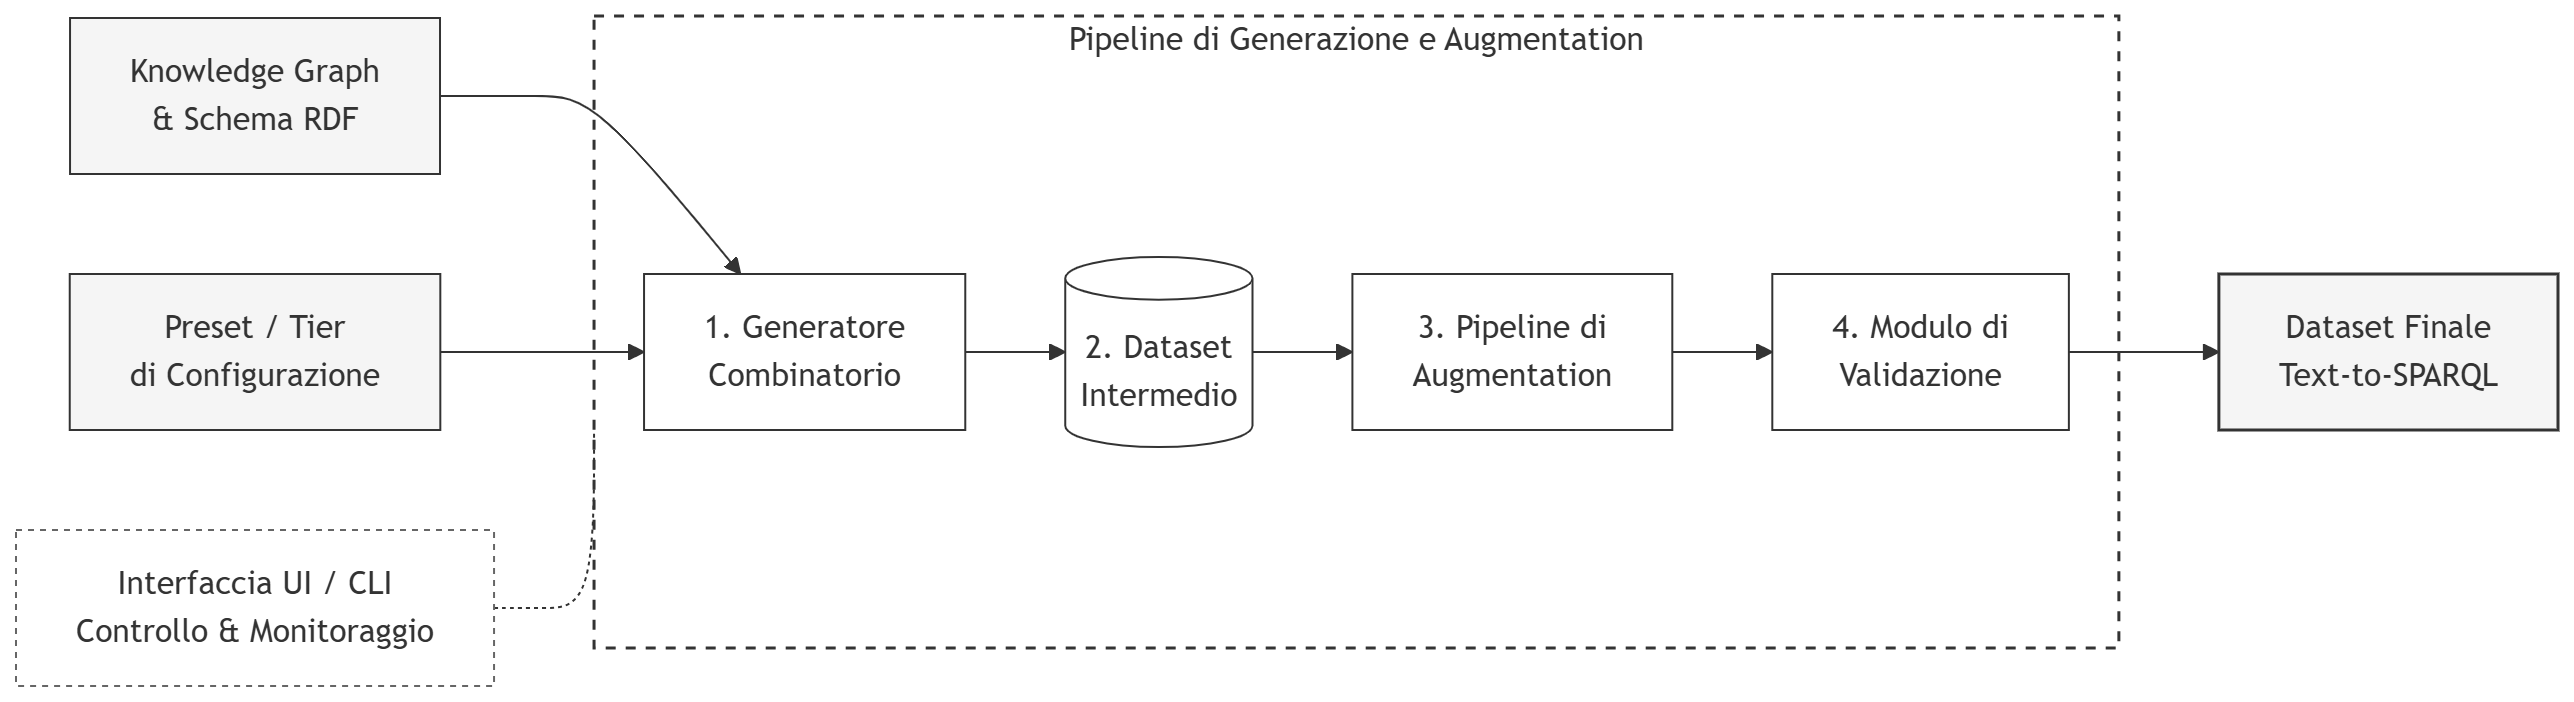
\includegraphics[width=\linewidth]{figures/pipeline-sample.png}
    \caption{Architettura macro ad alto livello della pipeline dati: flusso sequenziale dal Knowledge Graph fino alla validazione del dataset finale.}
    \label{fig:macro-architecture}
\end{figure}

\subsection{Modello del dominio}

Il modello di dominio di questo progetto non coincide con l'intero schema del
Knowledge Graph del Cancer Virtual Lab, ma con un sottoinsieme di 45 classi
fornito dall'IRST. La selezione delle classi non ha seguito un criterio
puramente tecnico o esaustivo, quale l'inclusione indiscriminata di ogni nodo
disponibile nel triplestore. Ma, al contrario, è stata strettamente guidata
dagli obiettivi clinici del progetto quali la costruzione di un dataset
focalizzato su query ad alta utilità operativa, ovvero capaci di rispecchiare i
quesiti informativi realmente posti da medici e ricercatori nella pratica
oncologica (quali l'individuazione di coorti di pazienti, il tracciamento dei
protocolli terapeutici e l'analisi della risposta ai trattamenti). Questo
sottoinsieme e la struttura relazionale che lo legano costituiscono un vincolo
imposto dal grafo ricevuto; di conseguenza, le decisioni progettuali affrontate
in questa sezione riguardano il modo in cui organizzare e pesare tali classi ai
fini della generazione, e non la scelta di quali includere.

Le 45 classi sono organizzate in gruppi di priorità decrescente
(\cref{fig:domain-model}) secondo un criterio di distanza strutturale dal nodo
\texttt{Patient}. L'adozione di tale metrica risponde a un'osservazione sul
dominio applicativo stesso: \texttt{Patient} costituisce la radice naturale del
grafo clinico, coerentemente con la modalità con cui un operatore sanitario
formula un quesito, ovvero a partire dall'entità paziente e non da una classe
periferica (quale può essere un singolo biomarcatore). La distanza dalla radice
offre un criterio oggettivo e calcolabile direttamente dalla topologia del
grafo, evitando l'imposizione arbitraria di un giudizio soggettivo sulla
rilevanza delle classi. Inoltre, tale misura rappresenta un'efficace
approssimazione della complessità delle query, basti pensare che una classe
raggiungibile con un solo passaggio relazionale genera tipicamente domande
dirette, mentre una classe raggiungibile con due o tre passaggi richiede query
che concatenano più relazioni, fornendo così un'indicazione sia sulla centralità
clinica sia sulla difficoltà attesa del quesito.

L'assenza di un criterio di priorizzazione avrebbe comportato conseguenze
dirette sul dataset prodotto, discusse in relazione a \hyperref[obj:O4]{O4} nel
capitolo di analisi. Trattando le 45 classi come equivalenti, il sistema avrebbe
allocato un budget di generazione identico a ciascuna. Di conseguenza, classi
concettualmente centrali quali \texttt{Patient}, \texttt{Diagnosis} e
\texttt{Therapy} avrebbero ottenuto una rappresentazione insufficiente rispetto
alla frequenza d'uso reale; al contrario, classi periferiche o altamente
granulari (come le singole categorie della classificazione TNM) avrebbero
prodotto un numero di esempi ridondante. Un simile sbilanciamento avrebbe
compromesso la capacità del modello addestrato di generalizzare in modo efficace
sulle categorie di domande più frequenti.

La distanza dal nodo \texttt{Patient} non costituisce l'unico criterio di
raggruppamento adottato. Un secondo schema, di natura tematica, organizza le
medesime 45 classi per area clinica (demografia, stadiazione, trattamento, ecc.)
ed è stato introdotto in una fase successiva, illustrata nel capitolo di
implementazione. I due criteri risultano complementari: la distanza strutturale
fornisce una progressione pulita di complessità per un primo passaggio di
generazione, mentre il raggruppamento tematico ricombina le classi secondo
relazioni di co-occorrenza differenti, consentendo a un secondo passaggio di
produrre query multi-relazionali strutturalmente nuove.

\begin{figure}[H]
    \centering
    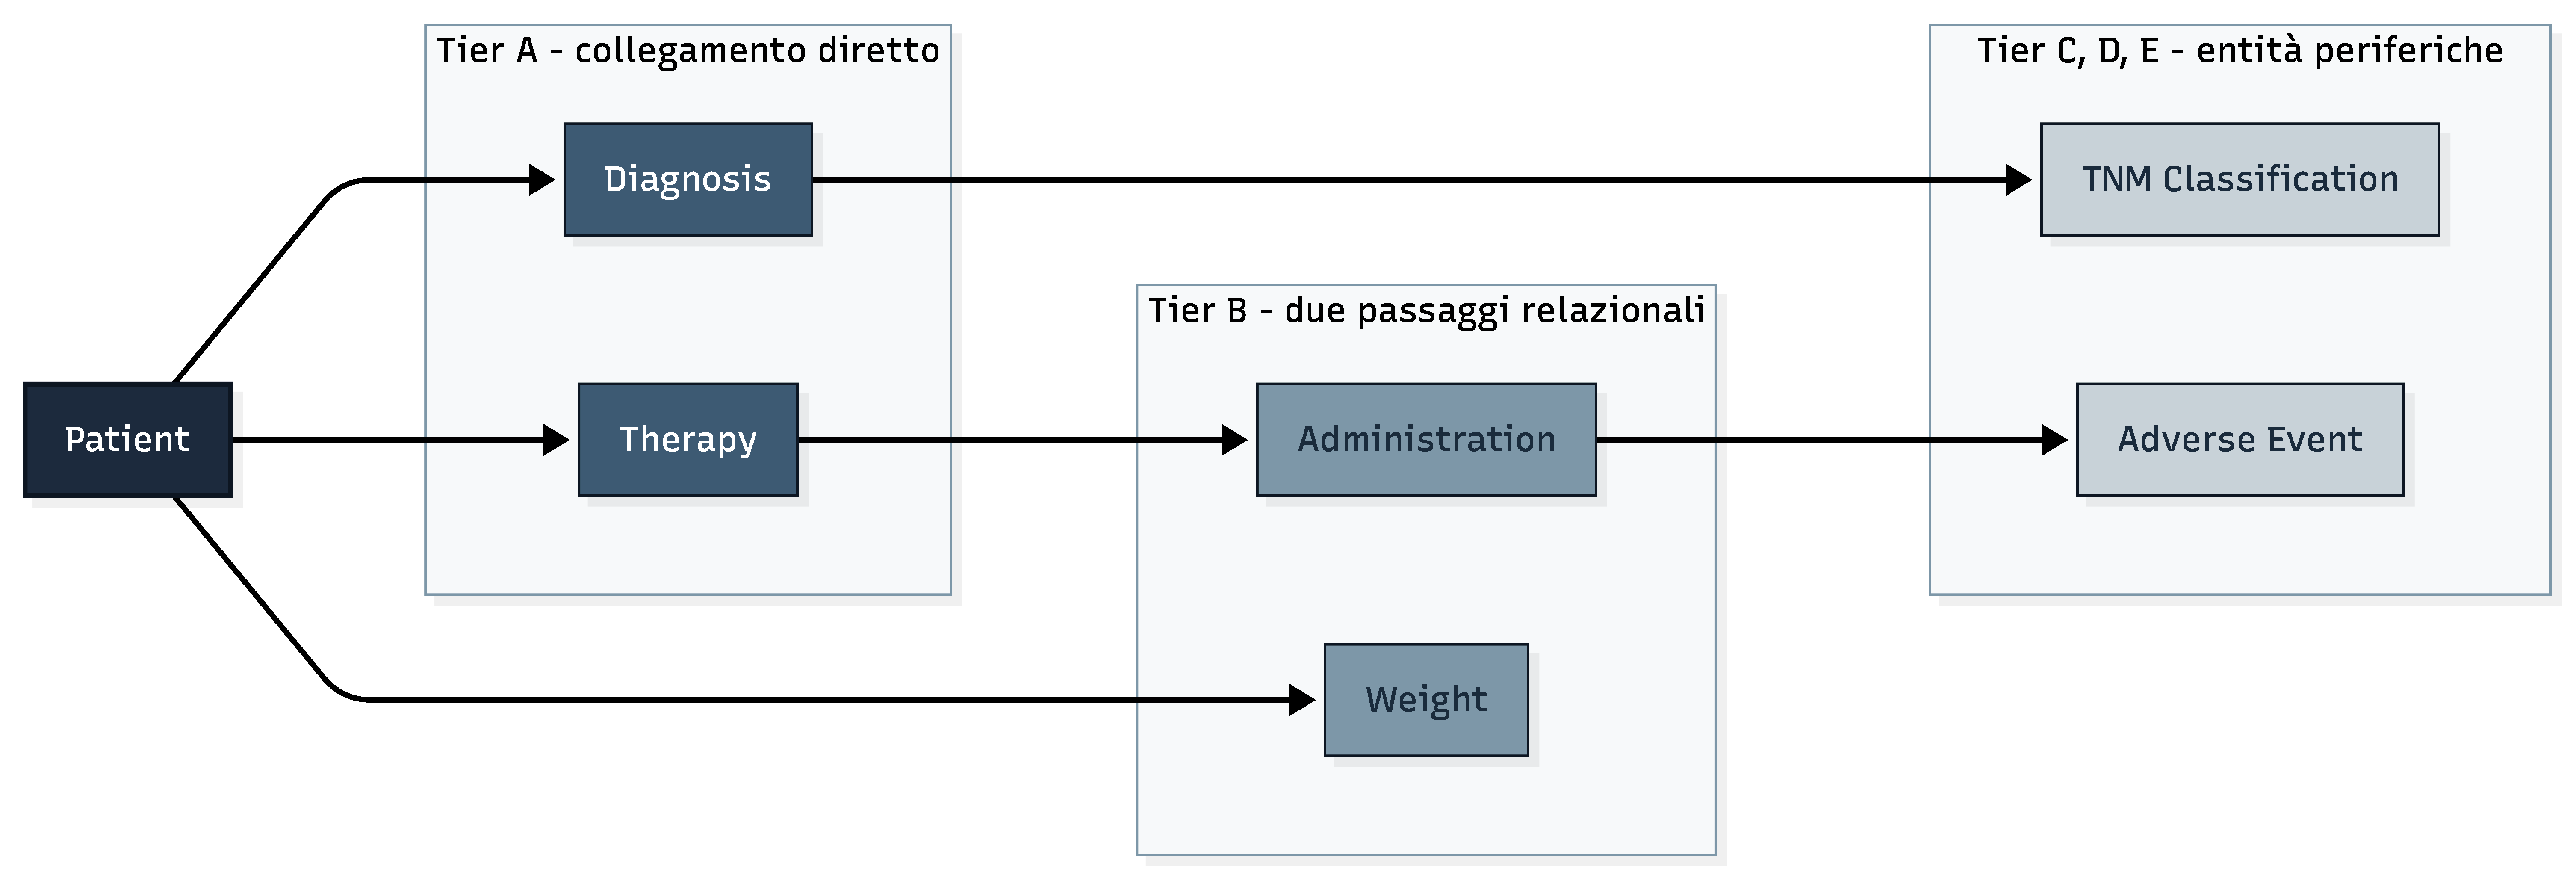
\includegraphics[width=.8\linewidth]{figures/domain-model-tiers.pdf}
    \caption{Modello di dominio semplificato, si noti Patient come nodo centrale}
    \label{fig:domain-model}
\end{figure}

Il numero di record generati per ciascun gruppo decresce dal centro alla
periferia del dominio, seguendo un andamento calibrato empiricamente per
bilanciare l'equilibrio finale del dataset, piuttosto che una formula matematica
definita a priori. Lo stesso principio di calibrazione empirica viene applicato
al sistema dei quattro parametri descritto nella sezione seguente.

In sintesi, il dataset Text-to-SPARQL prodotto non è generato in modo uniforme
sull'intero schema disponibile, ma rispetta una gerarchia di rilevanza clinica.
Le classi incluse e i parametri di complessità applicati riflettono le tipologie
di query ritenute prioritarie nel contesto del Cancer Virtual Lab, privilegiando
la pertinenza di dominio rispetto alla massimizzazione della copertura formale
del grafo.


\subsection{Sistema dei parametri}

Il modello di dominio descritto nella sezione precedente definisce quali classi
partecipano alla generazione e con quale peso relativo, ma non specifica in
alcun modo la complessità delle singole query generabili su ciascuna di esse.

Il generatore espone quattro parametri indipendenti, ciascuno regolabile entro
un intervallo minimo e massimo, la cui combinazione determina la complessità
della query risultante:

\begin{itemize}
    \item il numero di relazioni attraversate nel grafo a partire dal nodo
          radice;
    \item il numero di percorsi alternativi combinati nella medesima query
          tramite clausole di disgiunzione;
    \item il numero di proprietà vincolate su un medesimo nodo;
    \item il numero di valori ammessi per ciascun vincolo.
\end{itemize}

Disaccoppiare questi quattro parametri consente di modulare la struttura della
query in modo mirato. In questo modo è possibile, ad esempio, aumentare la
profondità delle relazioni sul grafo senza necessariamente incrementare il
numero di filtri sui singoli nodi, evitando la generazione di query
strutturalmente sbilanciate o non calibrate per lo schema di destinazione.

\begin{figure}[H]
    \centering
    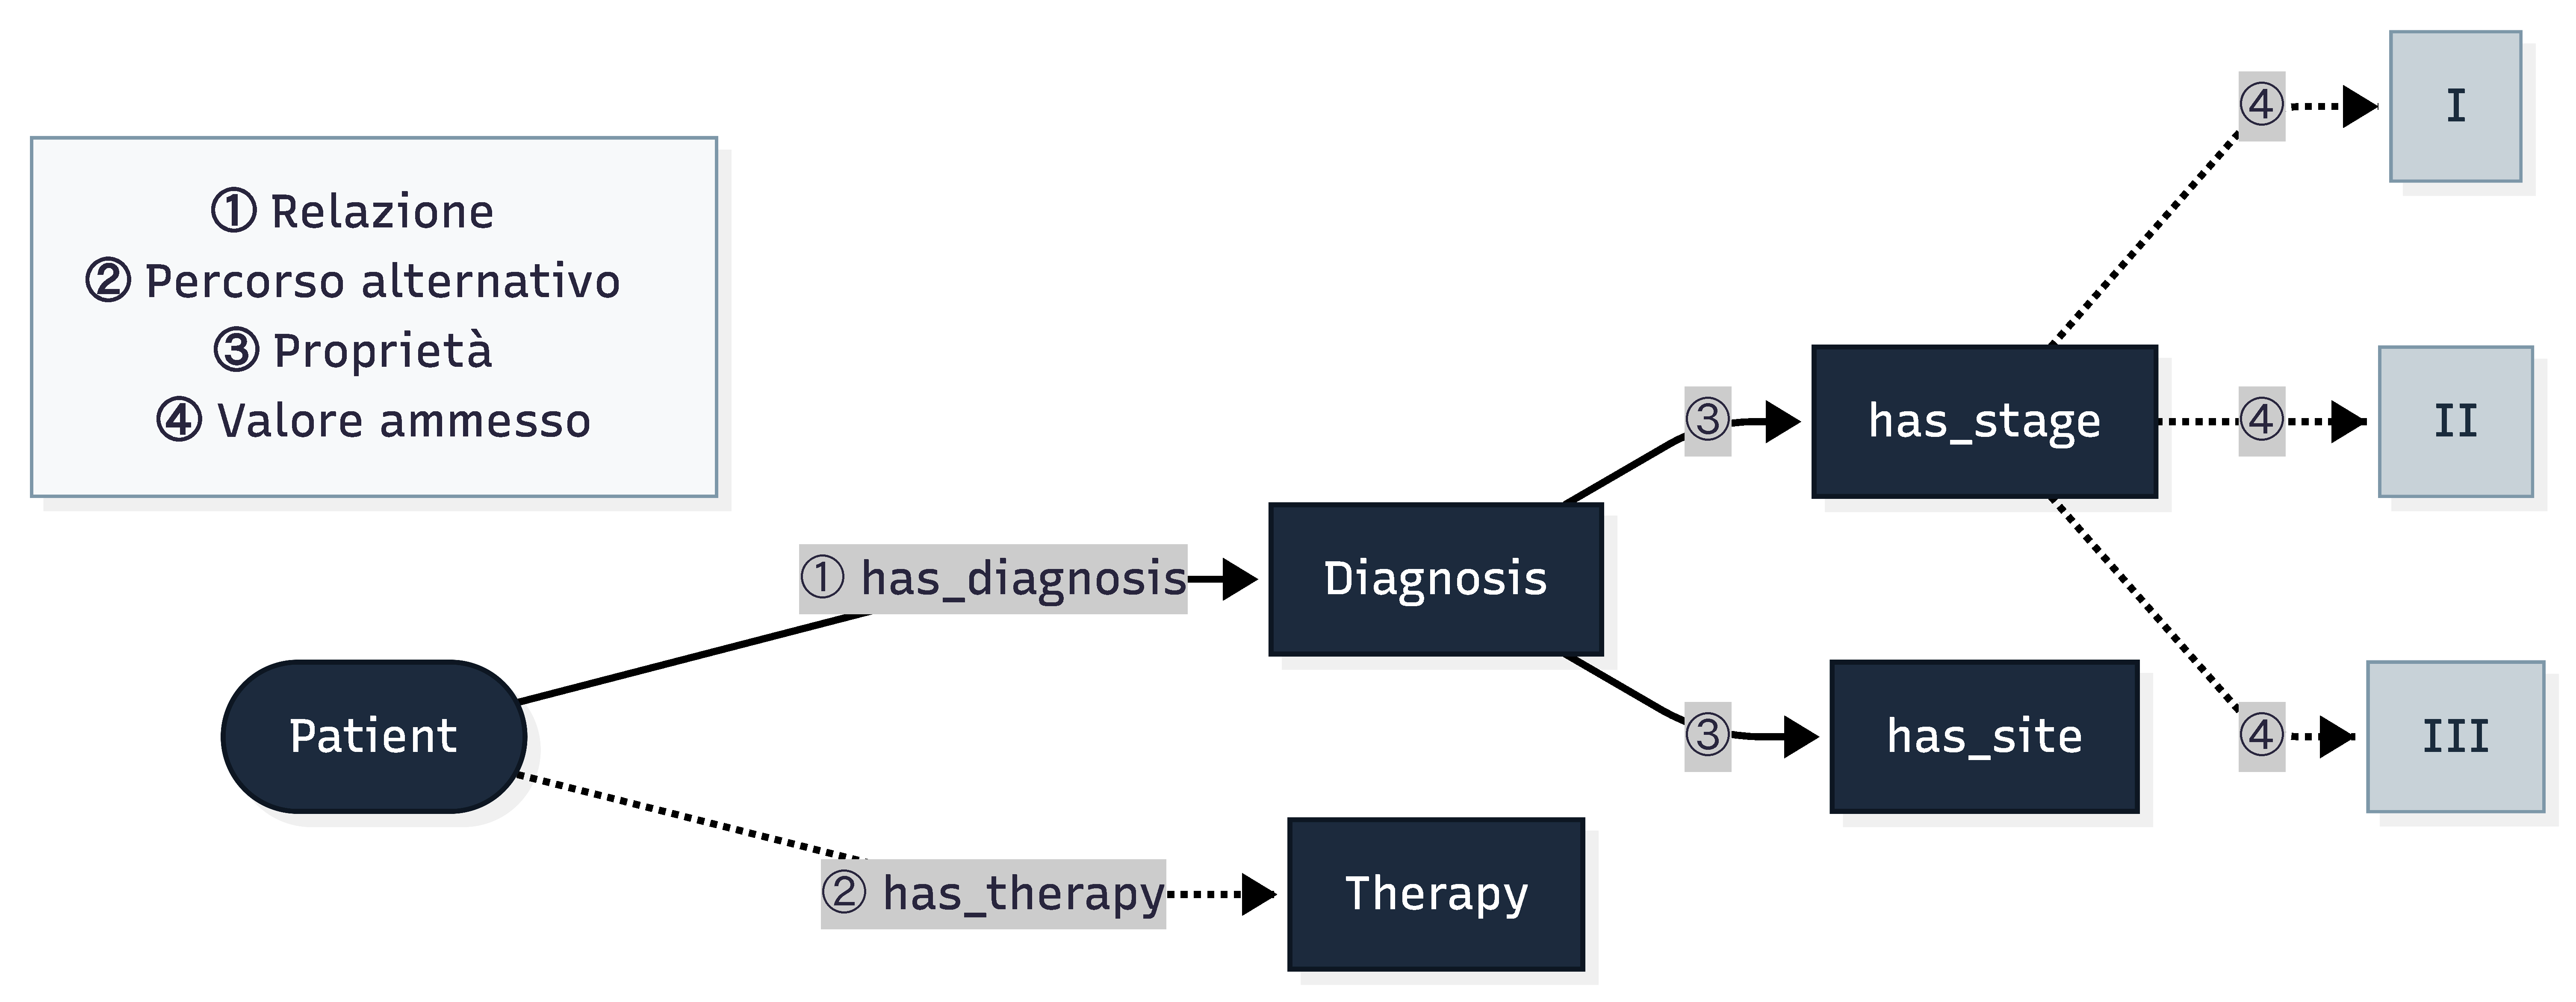
\includegraphics[width=.8\linewidth]{figures/generation-filters.pdf}
    \caption{Modello esemplificativo dei parametri filtrabili}
    \label{fig:generation filters}
\end{figure}

Sebbene l'impianto concettuale dei quattro parametri sia rimasto invariato nel
corso del progetto, i valori numerici effettivamente assegnati a ciascuno di
essi non sono stati definiti una sola volta, ma calibrati progressivamente
attraverso diverse configurazioni successive, tutte vincolate da un limite
superiore imposto dall'endpoint SPARQL stesso. Infatti query eccessivamente
complesse, al crescere del numero di relazioni e proprietà vincolate
simultaneamente, incorrevano in timeout o fallivano l'esecuzione contro il
triplestore reale, rendendo necessario mantenere ciascun parametro entro un
tetto massimo compatibile con le capacità dell'endpoint.

\subsection{Meccanismo di estensione incrementale}

Oltre a calibrare la complessità delle query, la struttura del sistema di
parametri supporta l'estensione incrementale del dataset. Questa proprietà
consente di integrare nuovi esempi in momenti successivi senza dover rielaborare
le porzioni già generate e garantendo l'assenza di sovrapposizioni con il corpus
esistente.

Il meccanismo si basa sulla definizione di regioni disgiunte all'interno dello
spazio parametrico. Poiché ciascun parametro (profondità, disgiunzioni,
proprietà e valori) è vincolato da un intervallo minimo e massimo, è possibile
configurare un nuovo \textit{preset} di generazione impostando intervalli
distinti da quelli usati in precedenza su almeno una dimensione. Così facendo,
il nuovo ciclo di generazione esplora esclusivamente combinazioni strutturali
mai campionate prima.

In fase di progettazione, questa separazione garantisce l'estensibilità del
sistema a due livelli:
\begin{itemize}
    \item \textbf{Estensione parametrica:} permette di ampliare il volume di
          dati definendo nuovi file di configurazione (\textit{tier}) esterni,
          senza modificare il codice sorgente del generatore;
    \item \textbf{Verifica dei duplicati:} l'assenza di sovrapposizioni
          garantita a livello teorico dalle configurazioni viene ulteriormente
          verificata durante la generazione, scartando eventuali query identiche
          prodotte per coincidenza stocastica.
\end{itemize}

L'aggiunta di nuove porzioni al dataset non richiede quindi una riprogettazione
dell'architettura, ma la semplice definizione di nuovi file di configurazione i
cui intervalli siano scelti in modo complementare rispetto a quelli già
esplorati.

\section{Design dell'augmentation}

Questa sezione descrive le decisioni progettuali alla base del secondo stadio
del sistema, responsabile della trasformazione delle coppie prompt-query
prodotte dal generatore in più varianti linguistiche naturali, secondo il
compromesso tra varietà e fedeltà semantica richiesto da \hyperref[obj:O2]{O2} e
la robustezza semantica richiesta da \hyperref[rnf:RNF3]{RNF3}.

\subsection{Mascheramento dei valori letterali e strategie di preservazione}

Il secondo stadio della pipeline affronta la sfida di bilanciare due requisiti
contrastanti individuati nella fase di analisi; da un lato massimizzare la
varietà linguistica dei prompt per evitare formulazioni rigide
(\hyperref[obj:O2]{O2}, \hyperref[rf:RF2]{RF2}), dall'altro garantire la rigida
fedeltà semantica e la preservazione dei valori clinici rispetto alla query
SPARQL associata (\hyperref[rf:RF3]{RF3}, \hyperref[rnf:RNF3]{RNF3}).

Lasciare che un modello linguistico riscriva liberamente l'intero testo, valori
compresi, esporrebbe il sistema ai rischi già identificati nel
\cref{chap:analisi}, quali l'alterazione o la perdita silenziosa di
identificativi, codici di classificazione o date.

Per risolvere questo problema, l'architettura adotta un pattern di mascheramento
deterministico che disaccoppia la struttura sintattica dai dati puntuali. Prima
di interpellare il modello, ogni valore letterale referenziato nella query viene
sostituito da un token segnaposto opaco (es. \texttt{[VAL\_A1B2]}). Il modello
opera così esclusivamente sulla componente sintattica e relazionale della frase,
privo di accesso ai dati reali, i quali vengono ripristinati solo al termine
della generazione. In questo modo si garantisce per costruzione che la
riformulazione non possa modificare i valori target.

Per superare i limiti espressivi e computazionali del mascheramento rigido, il
design del modulo integra due strategie specifiche:

\begin{itemize}
    \item \textbf{Traduzione proposizionale dei vincoli booleani:} Trattare i
          valori booleani come semplici stringhe letterali (es. \texttt{"true"}
          o \texttt{"false"}) produrrebbe prompt mascherati innaturali e
          sintatticamente rigidi. In fase di design si è stabilito di convertire
          i vincoli booleani, prima del mascheramento, in forme proposizionali
          naturali (es. trasformando una condizione su un evento avverso nelle
          preposizioni «con» o «senza» seguite dal termine clinico). Questa
          scelta risolve il problema della naturalezza espressiva senza delegare
          al modello la gestione del valore di verità.

    \item \textbf{Decomposizione in porzioni ad alta densità (C nking):}
          All'aumentare del numero di segnaposto in un singolo prompt, la
          capacità del modello di conservare ed elaborare tutti i token opachi
          degrada, aumentando il tasso di allucinazioni o l'omissione
          involontaria di segnaposto. Per mitigare questo limite, il sistema
          applica un principio di decomposizione: i prompt con un numero di
          segnaposto superiore a una soglia prestabilita vengono suddivisi in
          porzioni logiche indipendenti (\textit{chunk}), ciascuna contenente un
          budget limitato di token. Ogni porzione viene parafrasata
          separatamente e ricomposta nel testo finale, garantendo un tasso di
          accettazione elevato anche per query ad alta complessità combinatoria.
\end{itemize}

\subsection{Generazione iterativa e validazione}

Il mascheramento garantisce che i valori letterali, se presenti nell'output,
siano corretti; non garantisce però che il modello produca sempre un output
valido al primo tentativo, né che varianti successive dello stesso record non
finiscano per ripetersi tra loro, vanificando l'obiettivo di varietà linguistica
di \hyperref[obj:O2]{O2}.

Il sistema affronta questo problema attraverso un ciclo iterativo di generazione
e verifica. Ogni candidato prodotto dal modello viene sottoposto a una fase di
validazione che considera diversi criteri.

\begin{itemize}
    \item \textbf{Preservazione dei segnaposto.} Il candidato viene rifiutato se
          anche un solo segnaposto è stato omesso, modificato o sostituito.

    \item \textbf{Assenza di segnaposto non previsti.} Viene verificato che il
          testo non contenga sequenze che imitano la sintassi di un segnaposto
          senza corrispondere a uno dei segnaposto effettivamente presenti nel
          testo originale.

    \item \textbf{Controllo della similarità.} Il candidato viene confrontato
          con le varianti già accettate per lo stesso record. Se risulta
          eccessivamente simile a una di esse, viene rifiutato. La soglia di
          similarità viene resa progressivamente più permissiva al diminuire
          della lunghezza del testo, così da evitare che formulazioni brevi
          vengano considerate erroneamente come duplicati.
\end{itemize}

In caso di rifiuto, il sistema non si limita a ripetere la generazione. Il
candidato scartato e il relativo motivo vengono forniti al modello come contesto
aggiuntivo per il tentativo successivo, in modo da ridurre la probabilità che
venga ripetuto lo stesso errore. A ogni nuovo tentativo viene inoltre
incrementata progressivamente la temperatura di campionamento, favorendo la
produzione di una formulazione diversa da quella precedente.

Se anche l'ultimo tentativo disponibile viene rifiutato, il sistema non forza
comunque l'inserimento di una nuova variante. Viene invece mantenuto il testo
originale non modificato e viene registrato esplicitamente il ricorso a questo
comportamento di ripiego. In questo modo si evita di accettare silenziosamente
una formulazione che violi i vincoli definiti da \hyperref[rf:RF3]{RF3} o
\hyperref[rnf:RNF3]{RNF3}.

Inoltre, il budget di varianti target assegnato a ciascun record non viene
definito in modo uniforme, ma calcolato dinamicamente tramite una funzione
proporzionale alla densità di valori mascherati presenti nel prompt. Un testo
caratterizzato da un numero ridotto di vincoli presenta uno spazio di
variabilità linguistica ristretto; imporre una quota fissa di varianti a prompt
semplici avrebbe generato un'elevata frequenza di rigetti per eccessiva
similarità lessicale, saturando inutilmente il ciclo di tentativi e degradando
l'efficienza complessiva del processo (\hyperref[rnf:RNF1]{RNF1}). L'adozione di
una soglia adattiva garantisce quindi che la pressione generativa sia
concentrata sui record ad alta complessità combinatoria, massimizzando la
varietà utile ed evitando cicli di retry ridondanti sui casi più semplici.

\subsection{Varietà stilistica}

Il solo mascheramento non garantisce, di per sé, la varietà linguistica
richiesta da \hyperref[obj:O2]{O2}, anzi un modello lasciato libero di
riformulare tenderebbe a convergere su un piccolo numero di strutture
sintattiche ricorrenti. Il sistema affronta questo problema definendo un insieme
di dieci registri stilistici predefiniti (ad esempio una formulazione tecnica in
stile interrogazione a database, una clinico-formale, una colloquiale, una
statistica orientata al conteggio), esplicitamente descritti al modello a ogni
chiamata.

\begin{table}[H]
    \centering
    \small
    \renewcommand{\arraystretch}{1.2}
    \begin{tabularx}{\textwidth}{>{\bfseries}l X}
        \toprule
        Stile                & Formulazione della domanda                        \\
        \midrule
        Tecnico/SQL          & Estrai il conteggio totale dei record nella
        tabella pazienti che presentano la codifica 'Mammella femminile' e una
        data di nascita compresa nel range 01/01/1980 - 07/08/1995.              \\
        Clinico Formale      & Quanti soggetti di sesso femminile con diagnosi
        oncologica alla mammella risultano nati nel periodo compreso tra
        l'inizio del 1980 e il 7 agosto 1995?                                    \\
        Basato sull'età      & Fornisci il numero di pazienti con diagnosi
        'Mammella femminile' che hanno attualmente un'età compresa tra i 30 e i
        46 anni.                                                                 \\
        Gestionale/Reporting & Rapporto volumetrico: quante unità afferiscono
        alla patologia 'Mammella femminile' limitatamente alla coorte di nascita
        1980-1995 (fino al 7 agosto)?                                            \\
        Linguaggio Naturale  & Quante pazienti abbiamo in archivio che sono nate
        tra l'80 e metà agosto '95 e che soffrono di problemi alla mammella
        femminile?                                                               \\
        \bottomrule
    \end{tabularx}
    \caption{Esempio di variazione stilistica applicata a 5 registri rappresentativi a partire dal medesimo prompt mascherato.}
    \label{tab:style-variations-compact}
\end{table}

Gli stili non vengono assegnati alle varianti in modo casuale, ma percorsi in
sequenza ciclica, in modo che la distribuzione degli stili sulle varianti
generate risulti uniforme anziché soggetta alla variabilità di un'estrazione
casuale. Per ciascuno stile, il sistema mantiene inoltre una memoria a breve
termine delle formulazioni e delle parole di apertura usate più di recente, così
rifiutando eventuali nuovi candidati che riproponessere un'apertura già usata di
recente per lo stesso stile o una riformulazione troppo simile a livello di
intero testo, estendendo così il controllo di varietà anche alla struttura delle
prime parole della frase, non solo al suo contenuto complessivo.

Infine, per ciascun record il sistema conserva anche una formulazione di
controllo generata senza mascheramento, ottenuta inviando l'intero testo al
modello in un'unica richiesta diretta. Questa modalità non rappresenta un
percorso di produzione alternativo, bensì un punto di confronto semplice
(baseline) introdotto per misurare i reali benefici del mascheramento sulla
preservazione dei dati e sulla qualità del testo. La valutazione comparativa tra
i due approcci è trattata nella \cref{sec:eval-masking-comparison}.


\chapter{Implementazione}
\label{chap:implementation}

In questo capitolo viene descritto come sono state implementate le varie parti
del contributo di questa tesi, in maniera coerente con la progettazione svolta
nel \cref{chap:progettazione}. La trattazione segue l'ordine cronologico in cui
i due stadi del sistema sono stati sviluppati.

\section{Implementazione del generatore}
\label{sec:impl-generator}

\subsection{Architettura a mixin}
\label{sec:impl-mixin}

La pipeline di generazione descritta nel \cref{sec:design-pipeline} è realizzata
concretamente dalla classe \texttt{BulkDatasetGenerator}, la quale eredita
mediante ereditarietà multipla da sei \emph{mixin}, uno per ciascuna fase del
processo.

In coerenza con quanto introdotto nel \cref{sec:bg-software-tools}, questa
scelta architetturale applica il principio di singola responsabilità, garantendo
una corrispondenza diretta tra le fasi concettuali e i moduli software. Il
sistema espone così un'unica interfaccia orchestratrice per l'intero ciclo di
elaborazione, consentendo di modificare o estendere la logica di una specifica
fase intervenendo esclusivamente sul mixin dedicato, senza impattare sugli altri
componenti.

\begin{lstlisting}[
    language=Python,
    caption={Composizione della classe principale del generatore tramite mixin.},
    label={lst:mixin-composition}
]
class BulkDatasetGenerator(
    FilterApiMixin,
    DiscoveryMixin,
    SkeletonMixin,
    PlanningMixin,
    ProgressMixin,
    OutputMixin,
):
    # ...
\end{lstlisting}

Ciascun mixin realizza una o più delle fasi introdotte a livello di design,
incapsulando le chiamate di rete o coordinando la logica di più fasi quando
queste sono strettamente collegate tra loro:

\begin{itemize}
    \item \texttt{FilterApiMixin} incapsula le chiamate di rete verso l'API
          interna del CVL;

    \item \texttt{DiscoveryMixin} costruisce la mappa del grafo dello schema;

    \item \texttt{SkeletonMixin} costruisce lo scheletro di una singola query;

    \item \texttt{PlanningMixin} determina quali combinazioni di proprietà
          devono essere campionate;

    \item \texttt{OutputMixin} esegue i controlli di qualità finali e gestisce
          la scrittura dei risultati su disco;

    \item \texttt{ProgressMixin} gestisce gli aspetti legati all'interazione con
          l'interfaccia Streamlit, tra cui l'aggiornamento della barra di
          avanzamento e la possibilità di interrompere l'esecuzione.
\end{itemize}

Le responsabilità non sono quindi indipendenti, ma cooperano secondo il flusso
della generazione, ad eccezione di \texttt{ProgressMixin}, che costituisce
invece una responsabilità trasversale, poiché può intervenire durante
l'esecuzione delle diverse fasi senza rappresentare una fase autonoma della
pipeline.

La separazione è particolarmente evidente nella gestione dell'interruzione della
generazione (gestita proprio da \texttt{ProgressMixin}). Il metodo
\texttt{\_is\_aborted()}, riportato nel \cref{lst:abort}, viene richiamato
periodicamente durante la generazione per verificare se l'esecuzione debba
essere interrotta.

\begin{lstlisting}[
    language=Python,
    caption={Controllo dell'interruzione durante la generazione.},
    label={lst:abort}
]
def _is_aborted(self) -> bool:
    if self._abort_event.is_set():
        return True
    if not self.config.get("abortable", True):
        return False
    if self._can_paint() and bool(
        st.session_state.get("abort_generation", False)
    ):
        self._abort_event.set()
    return self._abort_event.is_set()
\end{lstlisting}

Il controllo appena citato combina due meccanismi:
\begin{itemize}
    \item l'evento di sincronizzazione interno \texttt{\_abort\_event}, che
          rappresenta lo stato di interruzione del run
    \item  lo stato dell'interfaccia Streamlit, dal quale viene letto il valore
          di \texttt{session\_state["abort\_generation"]}
\end{itemize}
Quando l'utente richiede l'interruzione, il metodo imposta l'evento interno; le
chiamate successive possono quindi rilevare direttamente tale stato senza dover
interrogare nuovamente l'interfaccia.

Il controllo dello stato di Streamlit viene eseguito soltanto quando
l'esecuzione è configurata come interrompibile, tramite
\texttt{config["abortable"]}, e quando il contesto consente di interagire con
l'interfaccia. In questo modo la stessa implementazione può essere utilizzata
anche nei contesti che non espongono un controllo di interruzione, come le
esecuzioni da riga di comando o un pannello di generazione batch.

Le costanti di classe di \texttt{BulkDatasetGenerator}, riportate nel
\cref{lst:mixin}, definiscono alcuni parametri di funzionamento condivisi dalle
diverse fasi della generazione.

\begin{lstlisting}[
    language=Python,
    caption={Costanti di classe utilizzate dal generatore.},
    label={lst:mixin}
]
class BulkDatasetGenerator(
    # parameters
):
    BUFFER_SIZE = 50
    MAX_DISCOVERY_WORKERS = 8
    GENERATION_WORKERS = 4
    DISCARD_SAMPLES = 500
    VALUE_REROLLS = 4
    MAX_STORED_VALUES = 5000
    SAMPLING_GIVEUP_STREAK = 250
\end{lstlisting}

In particolare, tali parametri controllano la dimensione del buffer di
scrittura, il grado di parallelismo utilizzato durante la scoperta e la
generazione, il numero massimo di valori conservati per proprietà e la soglia di
tentativi consecutivi senza successo oltre la quale il campionamento viene
interrotto. A questi si aggiungono i parametri relativi alla resilienza delle
chiamate di rete, costituiti da un timeout di base di 15 secondi, fino a due
ripetizioni in caso di fallimento e un secondo di attesa tra un tentativo e
l'altro (NON presenti nel \cref{lst:mixin}).

\subsection{Costruzione e indicizzazione della mappa del grafo}
\label{sec:impl-discovery}

Per evitare che l'esplorazione dello schema sia vincolata dai tempi di latenza
dell'I/O di rete, la fase di avvio esegue una scansione preliminare
dell'ontologia tramite il modulo \texttt{DiscoveryMixin}. Il risultato viene
strutturato in un dizionario Python in memoria (\texttt{graph\_map}), che agisce
da cache offline locale per l'intera esecuzione.

Come mostrato nel \cref{lst:graph-map}, l'implementazione organizza i dati
mediante due tabelle hash annidate, create separatamente per le proprietà
filtrabili e per le relazioni uscenti di ciascuna classe.

\begin{lstlisting}[
    language=Python,
    caption={Struttura della mappa del grafo memorizzata in \texttt{graph\_map}.},
    label={lst:graph-map}
]
graph_map = {
    "properties": {
        "Patient": [
            {
                "predicate": {"value": "has_gender", "label": "gender"},
                "datatype": "string",
                "n_values": 2,
                "values": [
                    {"value": "F", "label": "Female"},
                    {"value": "M", "label": "Male"}
                ]
            }
        ]
    },
    "relations": {
        "Patient": [
            {
                "predicate": {"value": "has_diagnosis", "label": "diagnosis"},
                "target": {"value": "Diagnosis", "label": "Diagnosis"}
            }
        ]
    }
}
\end{lstlisting}

La scelta di questa struttura dati e le relative modalità di popolamento
rispondono a tre precise esigenze implementative:

\begin{itemize}
    \item \textbf{Accesso in tempo costante $\mathcal{O}(1)$ durante la DFS:}
          Durante la ricerca in profondità dei percorsi
          (\cref{sec:impl-routes}), l'indicizzazione per chiave di entità
          consente l'estrazione immediata di proprietà e relazioni, evitando la
          scansione sequenziale di una lista globale ($\mathcal{O}(N)$).

    \item \textbf{Gestione della memoria (\texttt{MAX\_STORED\_VALUES}):} Per i
          campi ad alta cardinalità (es. misurazioni continue), il
          \texttt{DiscoveryMixin} applica un limite rigido alla lista
          \texttt{values}, memorizzando unicamente un campionario
          rappresentativo per la successiva fase di iniezione.


    \item \textbf{Parallelizzazione dell'I/O
              (\texttt{MAX\_DISCOVERY\_WORKERS}):} Poiché le chiamate REST per
          la scoperta delle singole entità sono operazioni indipendenti, il
          recupero iniziale può essere velocizzato sfruttando un pool di
          thread tramite
          \texttt{concurrent.futures.ThreadPoolExecutor}\footnote{\url{https://docs.python.org/3/library/concurrent.futures.html\#threadpoolexecutor}}.
\end{itemize}

L'uso di una mappa statica, però, introduce un'approssimazione di dominio: Il
sistema infatti assume che le proprietà di una classe dipendano unicamente dal
suo tipo e non dalla sequenza di salti relazionali con cui viene raggiunta, al
contrario rispetto l'API di CVL, la quale adotta un comportamento dinamico che
mostra o nasconde determinati vincoli in base allo storico della selezione.

Questa scelta progettuale è stata deliberatamente accettata a seguito di
un'analisi di fattibilità:

\begin{itemize}
    \item \textbf{Abbattimento della latenza di rete:} Senza la mappa in
          memoria, ogni nodo della DFS richiederebbe un'interrogazione HTTP
          sincrona. Nelle strutture ad alta complessità combinatoria, il volume
          di chiamate aumenterebbe in modo moltiplicativo, portando i tempi di
          generazione da pochi minuti a diverse ore con un alto rischio di
          timeout.

    \item \textbf{Impatto marginale sulla copertura (\hyperref[obj:O1]{O1}):} La
          mancata tracciabilità del contesto dinamico priva il sistema solo di
          predicati altamente specialistici legati a combinazioni rare,
          preservando appieno la rappresentazione delle query più frequenti e
          rilevanti per il dominio clinico.
\end{itemize}
\subsection{Costruzione delle route}
\label{sec:impl-routes}

Con la mappa disponibile, per ciascuna entità radice richiesta, si esplora
tramite una visita in profondità (DFS) ogni combinazione raggiungibile di salti
relazionali fino a un limite di profondità configurato.

\begin{lstlisting}[language=Python, caption={Visita in profondità della mappa del grafo per la costruzione delle route disponibili a partire da un'entità radice.}, label={lst:dfs}]
def dfs(type_value, chain, relations_used, visited, ancestor_terminals):
    terminals = [ {"predicate": p["predicate"], "chain_prefix": list(chain),
    ...} for p in properties.get(type_value, []) ] if terminals: routes.append({
    "chain": list(chain), "terminals": ancestor_terminals + [{**t,
    "is_final_entity": True} for t in terminals], })

    if relations_used >= max_relations: return inherited = ancestor_terminals +
        [{**t, "is_final_entity": False} for t in terminals] for rel in
        relations.get(type_value, []): target_value = (rel.get("target") or
        {}).get("value") if not target_value or target_value in visited:
        continue dfs( target_value, [*chain, {"predicate": rel["predicate"],
        "reference_to": rel.get("target")}], relations_used + 1, visited |
        {target_value}, inherited, )
\end{lstlisting}

Ogni volta che la visita raggiunge un nodo con proprietà filtrabili, viene
registrata una \emph{route}, ovvero l'insieme di:

\begin{itemize}
    \item la sequenza di salti relazionali per raggiungerlo (la \emph{chain});
    \item l'insieme delle proprietà disponibili in quel punto (i
          \emph{terminal}), che include sia quelle del nodo corrente sia quelle
          ereditate dai nodi attraversati in precedenza.
\end{itemize}

La distinzione dei terminal in proprietà ereditate e non (tramite variabile
booleana) garantisce, nel passo successivo di campionamento, che ogni
combinazione di proprietà scelta includa almeno un vincolo sul nodo in cui la
route si ferma davvero, evitando di costruire query che vincolano solo nodi di
passaggio.

Sebbene la visita che le genera sia intrinsecamente ad albero, l'insieme delle
route risultanti viene appiattito in una singola lista di record indipendenti
per facilitare la fase di campionamento (\cref{sec:impl-planning}), la quale
deve poter scorrere ed estrarre a caso qualunque route tra tutte quelle
disponibili, con accesso diretto e costante a ciascuna, senza dover ripercorrere
un albero ogni volta per ricostruire chain e terminal di un nodo scelto
casualmente al suo interno.

\subsection{Pianificazione: stima combinatoria e campionamento}
\label{sec:impl-planning}

Prima di generare i record, il sistema calcola quante coppie prompt-query
distinte siano effettivamente raggiungibili con le route disponibili e i vincoli
configurati, in modo da non richiedere più record di quanti lo spazio
combinatorio possa realmente offrire; solo dopo, campiona a caso tra le
combinazioni così stimate per costruire ogni singolo record.

\subsubsection{Stima combinatoria}

Sia $r$ una route, $T_r$ l'insieme dei suoi terminal e $T_r^f \subseteq T_r$ i
terminal finali (quelli del nodo dove la route si ferma davvero). Sia $v(t)$ il
numero di combinazioni di valori di un terminal, e $\mathcal{C}_k(T_r)$ le
combinazioni di $k$ terminal di $T_r$ (nel senso standard, $\binom{|T_r|}{k}$
possibilità) che includono almeno un terminal di $T_r^f$. Con
$\mathit{p_{\min}}$, $\mathit{p_{\max}}$ i limiti
$\mathit{min\_properties}$/$\mathit{max\_properties}$ configurati, il peso di
$r$ è

\begin{equation}
    \label{eq:route-weight}
    w(r) \;=\;
    \begin{cases}
        0 & \text{se } T_r^f = \emptyset \\[4pt]
        \displaystyle\sum_{k=\mathit{p_{\min}}}^{\min(\mathit{p_{\max}},\,|T_r|)}
        \;\sum_{c \,\in\, \mathcal{C}_k(T_r)} \;\prod_{t \,\in\, c} v(t)
          & \text{altrimenti.}
    \end{cases}
\end{equation}

Un record spesso combina più route insieme. Sia $V$ l'insieme delle route con
peso non nullo, e $\mathrm{indip}(S)$ vera quando nessuna coppia di route in $S$
ha una chain prefisso dell'altra (\cref{sec:impl-routes}). Con
$\mathit{s_{\min}}$, $\mathit{s_{\max}}$ i limiti
$\mathit{min\_paths}$/$\mathit{max\_paths}$ configurati, il tetto teorico
dell'entità è

\begin{equation}
    \label{eq:ceiling}
    N \;=\; \sum_{s=\mathit{s_{\min}}}^{\mathit{s_{\max}}}
    \;\sum_{\substack{S \subseteq V \\ |S|=s \\ \mathrm{indip}(S)}}
    \;\prod_{r \,\in\, S} w(r).
\end{equation}

È da sottolineare che $N$ è di fatto una sovrastima, in quanto route
indipendenti che condividono un prefisso condividono anche parte dei terminal,
mentre il prodotto dei pesi utilizzato nella nostra formula le tratta come
scelte separate. Per l'uso che se ne fa, cioè riconoscere quando lo spazio delle
combinazioni è troppo piccolo rispetto ai record richiesti, un limite superiore
basta, perciò possiamo evitare di complicare ulteriormente il calcolo. Proprio
per evitare un'ulteriore inefficienza, l'algoritmo imposta una soglia di
500\,000 combinazioni da esaminare, dopo la quale il conteggio esatto viene
abbandonato e il campionamento procede senza un tetto noto in anticipo.

\subsubsection{Campionamento}
\label{sec:impl-sampling}

Per ogni record da generare, il numero di route da combinare viene scelto a caso
entro i limiti configurati. Le route disponibili vengono poi estratte da un
elenco mescolato in ordine casuale, scartando quelle che risultano \emph{in
    conflitto} con una già scelta, cioè la cui chain è un prefisso di un'altra già
selezionata, il che indicherebbe due vincoli ridondanti sullo stesso tratto di
percorso. Il campionamento continua finché non si raggiunge il numero di record
stimato dal tetto teorico (\cref{eq:ceiling}), oppure finché 250 tentativi
consecutivi (\texttt{SAMPLING\_GIVEUP\_STREAK}) non producono nulla di nuovo,
segno che lo spazio raggiungibile è stato esaurito.

\begin{lstlisting}[language=Python, caption={Campionamento casuale di un insieme di route indipendenti tra loro per un singolo record.}, label={lst:sample-combo}]
def sample_independent_combo(target_p): pool = list(valid) rng.shuffle(pool)
    chosen, chosen_keys = [], [] for r in pool: if len(chosen) >= target_p:
    break key = chain_key_of[id(r)] if not routes_mod.conflicts(chosen_keys,
    key): chosen.append(r) chosen_keys.append(key) return tuple(chosen)
\end{lstlisting}

Questa modalità di campionamento casuale (\texttt{\_run\_sampled}) non è l'unica
prevista dal codice, esiste infatti anche una modalità a forza bruta
(\texttt{\_run\_brute\_force}) che enumera esaustivamente ogni combinazione
possibile di route e proprietà. Quest'ultima modalità risulta utile quando
l'obiettivo è ottenere una copertura completa dello spazio combinatorio;
tuttavia non è stata utilizzata nei run di produzione, ma è stata comunque
impiegata in fase di sviluppo per individuare eventuali errori di generazione,
proprio grazie alla sua capacità di esplorare lo spazio delle combinazioni senza
lasciarne fuori nessuna. Nella casistica affrontata da questa tesi però il
dataset generato è destinato al fine-tuning, per il quale non è necessario
enumerare tutte le combinazioni possibili, anzi è preferibile costruire un
insieme sufficientemente ampio e vario di esempi rappresentativi, evitando al
contempo di produrre una quantità di dati eccessiva rispetto allo scopo.

\subsection{Esecuzione sequenziale e parallela}
\label{sec:impl-execution}

Una volta pianificata una combinazione di route e proprietà da trasformare in un
record, ha inizio l'intero processo di costruzione del record vero e proprio, il
quale comporta diverse chiamate di rete verso l'API del CVL. Questo processo può
essere eseguito in sequenza, una combinazione alla volta, oppure in parallelo su
più thread, ciascuno impegnato a costruire un record diverso in contemporanea
agli altri, a seconda della configurazione.

\begin{lstlisting}[language=Python, caption={Scelta tra esecuzione sequenziale e parallela in base al numero di worker configurati.}, label={lst:workers}]
workers = max(1, int(self.config.get("num_workers") or self.GENERATION_WORKERS))
if workers <= 1: self._run_jobs_sequential(jobs_iter, total_pairs, p, target,
max_no_new) return
\end{lstlisting}

Se il numero di worker configurato è maggiore di uno, le combinazioni campionate
vengono sottomesse a un pool di thread, fino a \texttt{GENERATION\_WORKERS}
worker attivi contemporaneamente (di default 4), ciascuno impegnato nella
costruzione di un record indipendente. Il sistema non sottomette tuttavia tutte
le combinazioni disponibili in un'unica operazione, poiché ciò potrebbe
determinare l'accumulo in coda di un numero molto elevato di job in attesa.
Viene invece mantenuta una finestra di lavori sottomessi ma non ancora
completati, di dimensione pari al doppio del numero di worker attivi; quando la
generazione di un record termina e il risultato viene salvato, il relativo
spazio viene immediatamente riutilizzato per sottomettere una nuova
combinazione.

Questa strategia consente, in condizioni di parallelismo effettivo, di mantenere
i worker occupati riducendo i tempi morti, senza introdurre una quantità di
lavoro in coda eccessiva rispetto alla capacità di elaborazione disponibile. Il
meccanismo è stato predisposto principalmente in vista di future esecuzioni su
larga scala, nelle quali il parallelismo potrebbe ridurre significativamente il
tempo complessivo di generazione.

Durante la produzione del dataset trattato, il numero di worker è stato invece
impostato esplicitamente a 1 (\cref{lst:common-config}) eseguendo così la
generazione in modalità single-threaded. La scelta è dettata dal collo di
bottiglia rappresentato dalle chiamate all'API, le cui richieste concorrenti non
avrebbero ridotto i tempi in proporzione, anzi avrebbero rischiato di
comprometterne stabilità e prestazioni. Il parallelismo è rimasto invece attivo
nella scoperta della mappa (\cref{sec:impl-discovery}), dove il carico delle
operazioni si presta meglio all'esecuzione concorrente.

Proprio perché il parallelismo può comunque essere attivato lo stato condiviso
tra i thread non è protetto da un unico lock globale ma da quattro lock
distinti, ciascuno a guardia di una porzione di stato diversa e indipendente
dalle altre:
\begin{itemize}
    \item un lock protegge gli insiemi usati per riconoscere i duplicati
    \item un altro la cache dello scheletro (\cref{sec:impl-skeleton})
    \item un altro ancora le statistiche interne sulle chiamate effettuate
    \item l'ultimo il registro dei job attualmente in esecuzione
          (\cref{sec:impl-output})
\end{itemize}
Tenerli separati, invece di usarne uno solo per tutto, evita che un thread resti
bloccato in attesa di una struttura dati che non gli serve, solo perché un altro
thread ne sta aggiornando una diversa nello stesso istante.

\subsection{Costruzione dello scheletro: percorso online e offline}
\label{sec:impl-skeleton}

Ogni combinazione campionata deve essere tradotta in una struttura dati
intermedia, chiamata \emph{scheletro}, che rappresenta i nodi del grafo
coinvolti nella query, prima ancora che i valori concreti vengano scelti. Il
sistema offre due percorsi alternativi per costruirla, insieme ad altre opzioni
di comportamento, tutte raccolte in un'unica configurazione condivisa da
entrambe le liste di tier.

\subsubsection{Le opzioni condivise}
\label{sec:impl-config}

\begin{lstlisting}[language=Python, caption={Configurazione condivisa usata nei run di produzione, per entrambe le liste di tier.}, label={lst:common-config}]
COMMON_CONFIG = { "num_workers": 1, "offline_history": True,
    "include_value_spans": True, "skip_navigation_in_prompt": False,
    "validate_sparql": True, }
\end{lstlisting}

Ciascuna di queste cinque opzioni governa un aspetto distinto del comportamento
del generatore.

\begin{itemize}
    \item \texttt{num\_workers} a 1 è la scelta, già motivata in
          \cref{sec:impl-execution}, di eseguire la generazione in sequenza
          anziché in parallelo.
    \item \texttt{include\_value\_spans} controlla se il generatore debba
          tracciare le posizioni dei valori letterali nel prompt
          (\cref{sec:impl-phrasing}, dove è ripreso in dettaglio).
    \item \texttt{skip\_navigation\_in\_prompt}, se attivato ometterebbe dal
          testo del prompt le clausole di sola navigazione, rendendolo più corto
          ma meno esplicito sul percorso nel grafo; è stato tenuto disattivato
          in produzione per non perdere quell'informazione.
    \item \texttt{validate\_sparql} controlla se la query SPARQL restituita
          dall'API debba passare un controllo di sintassi prima di essere
          accettata; sarà ripreso più avanti insieme agli altri controlli di
          qualità (\cref{sec:impl-output}).
    \item \texttt{offline\_history} decide se lo scheletro venga ricostruito in
          locale oppure costruito camminando dal vivo dentro l'API; riguarda
          direttamente le due sottosezioni seguenti.
\end{itemize}

\subsubsection{Il percorso online}

Quando \texttt{offline\_history} è disattivato, lo scheletro viene costruito
camminando passo per passo tramite chiamate ricorsive nell'API del CVL,
esplorando in modo consequenziale proprietà e relazioni. Per ogni terminal della
combinazione, il sistema percorre uno per uno i salti della sua chain
(\cref{sec:impl-routes}) e, a partire dall'entità radice, a ogni salto chiede
all'API di proseguire dal nodo raggiunto fino a quel momento verso il nodo
successivo, accumulando progressivamente lo stato della query in costruzione
finché non raggiunge il nodo del terminal stesso. Questa procedura ripercorre
esattamente il percorso che la fase di scoperta della mappa aveva già seguito
per costruire la mappa iniziale (\cref{sec:impl-discovery}); la differenza è che
lì veniva fatto una volta per ogni proprietà isolata, mentre qui viene ripetuto
per intero a ogni singolo record. Durante questa fase di costruzione online sono
inoltre presenti alcuni meccanismi di resilienza, introdotti per gestire le
condizioni anomale e gli eventuali problemi che possono verificarsi durante le
chiamate all'API. Tali meccanismi si sono rivelati necessari nel corso dello
sviluppo e vengono descritti di seguito.

\begin{itemize}
    \item se l'API impiega troppo a rispondere, il fallimento è considerato
          transitorio, perché un tentativo successivo potrebbe ancora avere
          successo, e non viene memorizzato in nessuna cache;
    \item se invece risponde ma senza risultati utili, il terminal è considerato
          irraggiungibile in modo permanente, con due conseguenze distinte:
          \begin{itemize}
              \item viene memorizzato in una cache condivisa così che i
                    tentativi successivi lo scartino subito senza ripetere
                    l'esplorazione;
              \item il record in corso esclude dalla combinazione quel singolo
                    terminal e la generazione prosegue con gli altri rimasti
                    (esiste una modalità più rigida, mai usata in produzione,
                    che interromperebbe l'intero tentativo al primo terminal
                    irraggiungibile);
          \end{itemize}
    \item indipendentemente dai primi due, per non ripetere l'intera
          esplorazione quando la stessa combinazione di terminal ricorre in
          record diversi, lo scheletro completo viene tenuto in una cache
          separata, indicizzata sulla combinazione esatta richiesta, e riusato
          direttamente se si ripresenta, con solo il riempimento dei valori
          concreti (\cref{sec:impl-values}) che cambia da un record all'altro.
\end{itemize}

\subsubsection{Il percorso offline}

Con \texttt{offline\_history} attivo, come nei run di produzione, tutta la
camminata appena descritta viene saltata e lo scheletro non si costruisce
esplorando dal vivo l'API del CVL, ma viene ricostruito interamente in locale a
partire dai dati che la scoperta della mappa aveva già raccolto per ciascuna
proprietà (\cref{sec:impl-discovery}). Per ogni terminal coinvolto nella
combinazione, il sistema ricrea la stessa sequenza di nodi intermedi che
un'esplorazione dal vivo avrebbe prodotto, camminando sulla sequenza di salti
già nota (registrata al momento della scoperta delle route,
\cref{sec:impl-routes}) e usando i valori possibili già memorizzati per quel
terminal, senza doverli richiedere di nuovo; con lo scheletro pronto, si arriva
così direttamente all'unico passaggio che nessuno dei due percorsi può evitare,
ovvero la chiamata finale descritta di seguito.

\begin{lstlisting}[language=Python, caption={Lo scheletro appena ricostruito per i terminal \texttt{gender} e \texttt{birth date}, ancora privo di valori.}, label={lst:skeleton-example}]
history = [ { "query_nodes": [ {"predicate": {"label": "gender"}, "values":
    None, "value_range": None}, {"predicate": {"label": "birth date"}, "values":
    None, "value_range": None}, ] } ]
\end{lstlisting}

Indipendentemente dal percorso scelto per lo scheletro, il testo effettivo della
query SPARQL viene sempre ottenuto con un'unica chiamata finale all'API, che
traduce la struttura accumulata in una query eseguibile. Questo passaggio non è
mai eseguito localmente, in nessuna delle due modalità, rappresentando così
l'unica chiamata API fatta dal percorso offline. Su questa stessa chiamata
finale interviene anche il quinto flag di \cref{lst:common-config},
\texttt{validate\_sparql}, ripreso e motivato più avanti insieme agli altri
controlli di qualità applicati al risultato finale (\cref{sec:impl-output}).

\subsection{Riempimento dei valori}
\label{sec:impl-values}

Una volta pronto lo scheletro, ogni suo nodo vuoto viene riempito con valori
concreti scelti a caso dal pool associato al terminal corrispondente.

\begin{lstlisting}[language=Python, caption={Riempimento di un nodo dello scheletro con valori concreti, distinguendo tra intervalli e insiemi discreti.}, label={lst:fill-node}]
def fill_node(node, term, pool, min_values, max_values): k =
    random.randint(min_values, min(max_values, len(pool))) chosen =
    random.sample(pool, k) if _is_range_datatype(term.get("datatype")): ordered
    = sorted(chosen, key=lambda v: v["value"]) node["value_range"] = {"min":
    ordered[0]["value"], "max": ordered[-1]["value"]} else: node["values"] =
    chosen
\end{lstlisting}

Il numero di valori da usare per un dato vincolo è scelto a caso entro i limiti
configurati (\cref{lst:fill-node}), evitando però di selezionare l'intero
dominio possibile di un campo, perché un vincolo che copre tutti i valori
ammessi non escluderebbe di fatto nessun paziente, risultando così privo di
potere selettivo. Se il campo è una data o un valore numerico, i valori scelti
vengono usati per costruire un intervallo anziché un elenco discreto.

\begin{lstlisting}[language=Python, caption={Lo stesso scheletro di \cref{lst:skeleton-example}, dopo il riempimento: elenco discreto per il campo categoriale, intervallo per quello di tipo data.}, label={lst:filled-nodes}]
history = [ { "query_nodes": [ {"predicate": {"label": "gender"}, "values":
    [{"value": "F", "label": "Female"}], "value_range": None}, {"predicate":
    {"label": "birth date"}, "values": None, "value_range": {"min":
    "2016-01-01", "max": "2019-01-01"}}, ] } ]
\end{lstlisting}

\subsection{Generazione del prompt e tracciamento degli span}
\label{sec:impl-phrasing}

Definiamo un \textit{segmento} come un pezzo di testo accompagnato da un
booleano che indica se il testo contenga un valore letterale, come una data o un
codice, oppure solo una parola di struttura della frase come \emph{with} o
\emph{and}. Con lo scheletro completo di valori, il prompt viene costruito
riassemblando i suoi nodi in una lista di segmenti, concatenati uno via l'altro
formando il prompt finale. La formulazione di ciascun segmento dipende da cosa
contiene il nodo di origine:

\begin{itemize}
    \item se il nodo ha valori scelti (\cref{sec:impl-values}), il segmento
          inizia con \emph{with} seguito dai valori stessi, uniti da \emph{or}
          se sono due, o da una serie di virgole con un \emph{or} finale se sono
          di più;
    \item se rappresenta un intervallo, diventa \emph{between X and Y};
    \item un nodo senza valori propri, che serve solo a passare al nodo
          successivo della chain senza introdurre un vincolo, produce invece un
          segmento con \emph{which} al posto di \emph{with}; un nodo
          \emph{diagnosis} senza valori seguito da un nodo \emph{stage} con
          valore \emph{II} produce ad esempio \emph{"which diagnosis with stage
              II"}.
\end{itemize}

I segmenti di uno stesso passo della chain vengono uniti con un semplice
\emph{and}, e lo stesso connettivo lega tra loro i passi successivi, a partire
da un'apertura fissa (\emph{"Find all \textless entità\textgreater"}).

\begin{lstlisting}[language=Python, caption={Costruzione del prompt segmento per segmento, con tracciamento diretto della posizione di ciascun valore letterale.}, label={lst:build-prompt}]
def build_prompt_with_spans(root_label, history, skip_navigation=False):
    segments = _prompt_segments(root_label, history, skip_navigation) pieces,
    spans = [], [] for is_value, text in segments: if is_value: base =
    sum(len(p) for p in pieces) spans.append((base, base + len(text)))
    pieces.append(text) return "".join(pieces), spans
\end{lstlisting}

Mentre i segmenti vengono concatenati uno alla volta, la posizione di ciascun
valore inserito nel testo viene registrata. Determinare gli intervalli solo a
partire dal prompt finale sarebbe infatti ambiguo nel caso in cui lo stesso
valore comparisse, per coincidenza, anche in un'altra posizione della frase.
Registrare le coordinate durante la costruzione del testo elimina quindi questa
ambiguità senza richiedere controlli aggiuntivi. La funzione restituisce sempre
la coppia \texttt{(prompt, value\_spans)}, ma solo più avanti, al momento di
salvare il record completo, il flag \texttt{include\_value\_spans}
(\cref{sec:impl-config}) decide se il campo \texttt{value\_spans} venga scritto
nell'output finale o scartato (sempre attivo nei run di produzione).

Applicata allo scheletro pieno di \cref{lst:filled-nodes}, la procedura produce
il prompt \emph{"Find all patient with gender Female and birth date between
    2016-01-01 and 2019-01-01"}, con \texttt{value\_spans} pari a $[(29,35),
        (59,69), (74,84)]$, che corrispondono rispettivamente a \emph{"Female"},
\emph{"2016-01-01"} e \emph{"2019-01-01"}.

\subsection{Controlli di qualità e deduplicazione}
\label{sec:impl-output}

Prima della persistenza su disco, ogni coppia prompt-query generata viene
sottoposta a una sequenza di tre controlli di qualità indipendenti:

\begin{enumerate}
    \item \textbf{Verifica dell'effettiva applicazione dei filtri:} Il primo
          controllo accerta che la query SPARQL generata dall'API contenga le
          clausole \texttt{FILTER} o \texttt{VALUES}, oppure almeno uno dei
          valori letterali campionati. Questo passaggio intercetta le risposte
          anomale del backend che, pur restituendo una sintassi valida, ignorano
          i vincoli richiesti. Una query priva di filtri risulterebbe
          semanticamente decontestualizzata rispetto al prompt associato,
          introducendo un esempio errato nel dataset. Qualora nessuna condizione
          sia soddisfatta, il record viene scartato con la motivazione esplicita
          \emph{"the backend ignored our filters"}.

          \begin{lstlisting}[
        language=Python,
        caption={Verifica della presenza dei vincoli nella query SPARQL.},
        label={lst:filters-landed}
    ]
def _filters_landed(sparql, chosen_values):
    if "FILTER" in sparql or "VALUES" in sparql:
        return True
    return any(v in sparql for v in chosen_values)
    \end{lstlisting}

    \item \textbf{Parsing sintattico deterministico:} Il secondo controllo
          valida la correttezza formale della query tramite il parser della
          libreria \texttt{rdflib}. L'obiettivo è prevenire l'inclusione di
          query malformate che insegnerebbero al modello linguistico una
          grammatica errata. Il controllo è subordinato al parametro di
          configurazione \texttt{validate\_sparql} (\cref{lst:common-config}),
          abilitato nei run di produzione. Gli esempi che falliscono l'analisi
          sintattica vengono scartati con il motivo \emph{"the SPARQL does not
              parse (rdflib)"}.

          \begin{lstlisting}[
        language=Python,
        caption={Validazione sintattica condizionata della query SPARQL.},
        label={lst:validate-sparql}
    ]
syntax_error = (
    validate.sparql_error(sparql)
    if self.config.get("validate_sparql", True)
    else None
)
    \end{lstlisting}

    \item \textbf{Deduplicazione e rigenerazione dei valori:} L'ultimo controllo
          garantisce l'unicità dei dati mantenendo due tabelle hash in memoria:
          una contenente i prompt già accettati e una per gli digest calcolati
          sulle coppie prompt-query. In questo modo si evita che l'estrazione
          casuale generi combinazioni identiche di route e valori, le quali
          ridurrebbero la varietà reale del corpus. Qualora venga rilevato un
          prompt duplicato, il sistema esegue fino a 4 tentativi di
          rigenerazione dei valori (\texttt{VALUE\_REROLLS}) prima di scartare
          definitivamente il record.
\end{enumerate}

Le coppie che superano l'intero processo di validazione vengono accumulate in un
buffer di memoria e scritte su disco a blocchi di 50 elementi
(\texttt{BUFFER\_SIZE}).

\subsection{Generazione manuale a entità singola}
\label{sec:impl-manual}

L'architettura del sistema disaccoppia nettamente la logica del motore di
generazione finora descritto dalla sua modalità di invocazione. La classe
\texttt{BulkDatasetGenerator} è progettata per essere del tutto "inconsapevole"
del contesto di esecuzione, essa riceve infatti una semplice configurazione ed
esegue il flusso di generazione indipendentemente dall'interfaccia che la
richiama.

Per consentire l'interazione diretta con questo motore, nell'ambito di questo
lavoro di tesi è stato realizzato un pannello di controllo interattivo integrato
nella piattaforma CVL tramite il framework Streamlit. Tale modulo fornisce
un'interfaccia grafica per istanziare ed eseguire il generatore su una singola
entità radice, mettendo a disposizione 5 sezioni principali:

\begin{itemize}
    \item \textbf{Graph Map}: precondizione per tutto il resto, ha un pulsante
          che permette di caricare la mappa del grafo
          (\cref{sec:impl-discovery}) e ne mostra un riepilogo (numero di
          entità, proprietà e relazioni scoperte) una volta completata.
    \item \textbf{Mode}: sceglie tra questa modalità a entità singola e la
          generazione automatica da file di tier (\cref{sec:impl-tier-config}).
    \item \textbf{Starting Entity}: un menu a tendina per scegliere l'unica
          entità radice da cui far partire la generazione.
    \item \textbf{Configuration}: quattro slider, uno per relazioni da
          attraversare, proprietà per percorso, percorsi simultanei e valori per
          proprietà.
    \item \textbf{Generation Mode} e \textbf{History building}: espongono
          direttamente, tramite interruttori e caselle di spunta, parametri già
          discussi altrove in questo capitolo, come la scelta tra campionamento
          e forza bruta e il numero di worker
          (\cref{sec:impl-sampling,sec:impl-execution}), o i flag
          \texttt{offline\_history}, \texttt{include\_value\_spans},
          \texttt{skip\_navigation\_in\_prompt} (\cref{sec:impl-config}).
\end{itemize}

Gli estremi dei quattro slider di configurazione non sono fissi, ma vengono
calcolati a runtime scoprendo, tramite \texttt{discover\_routes\_from\_map}
(\cref{sec:impl-routes}), quante route siano effettivamente raggiungibili da
quell'entità con i limiti scelti.

%\begin{figure}[H] \centering
%    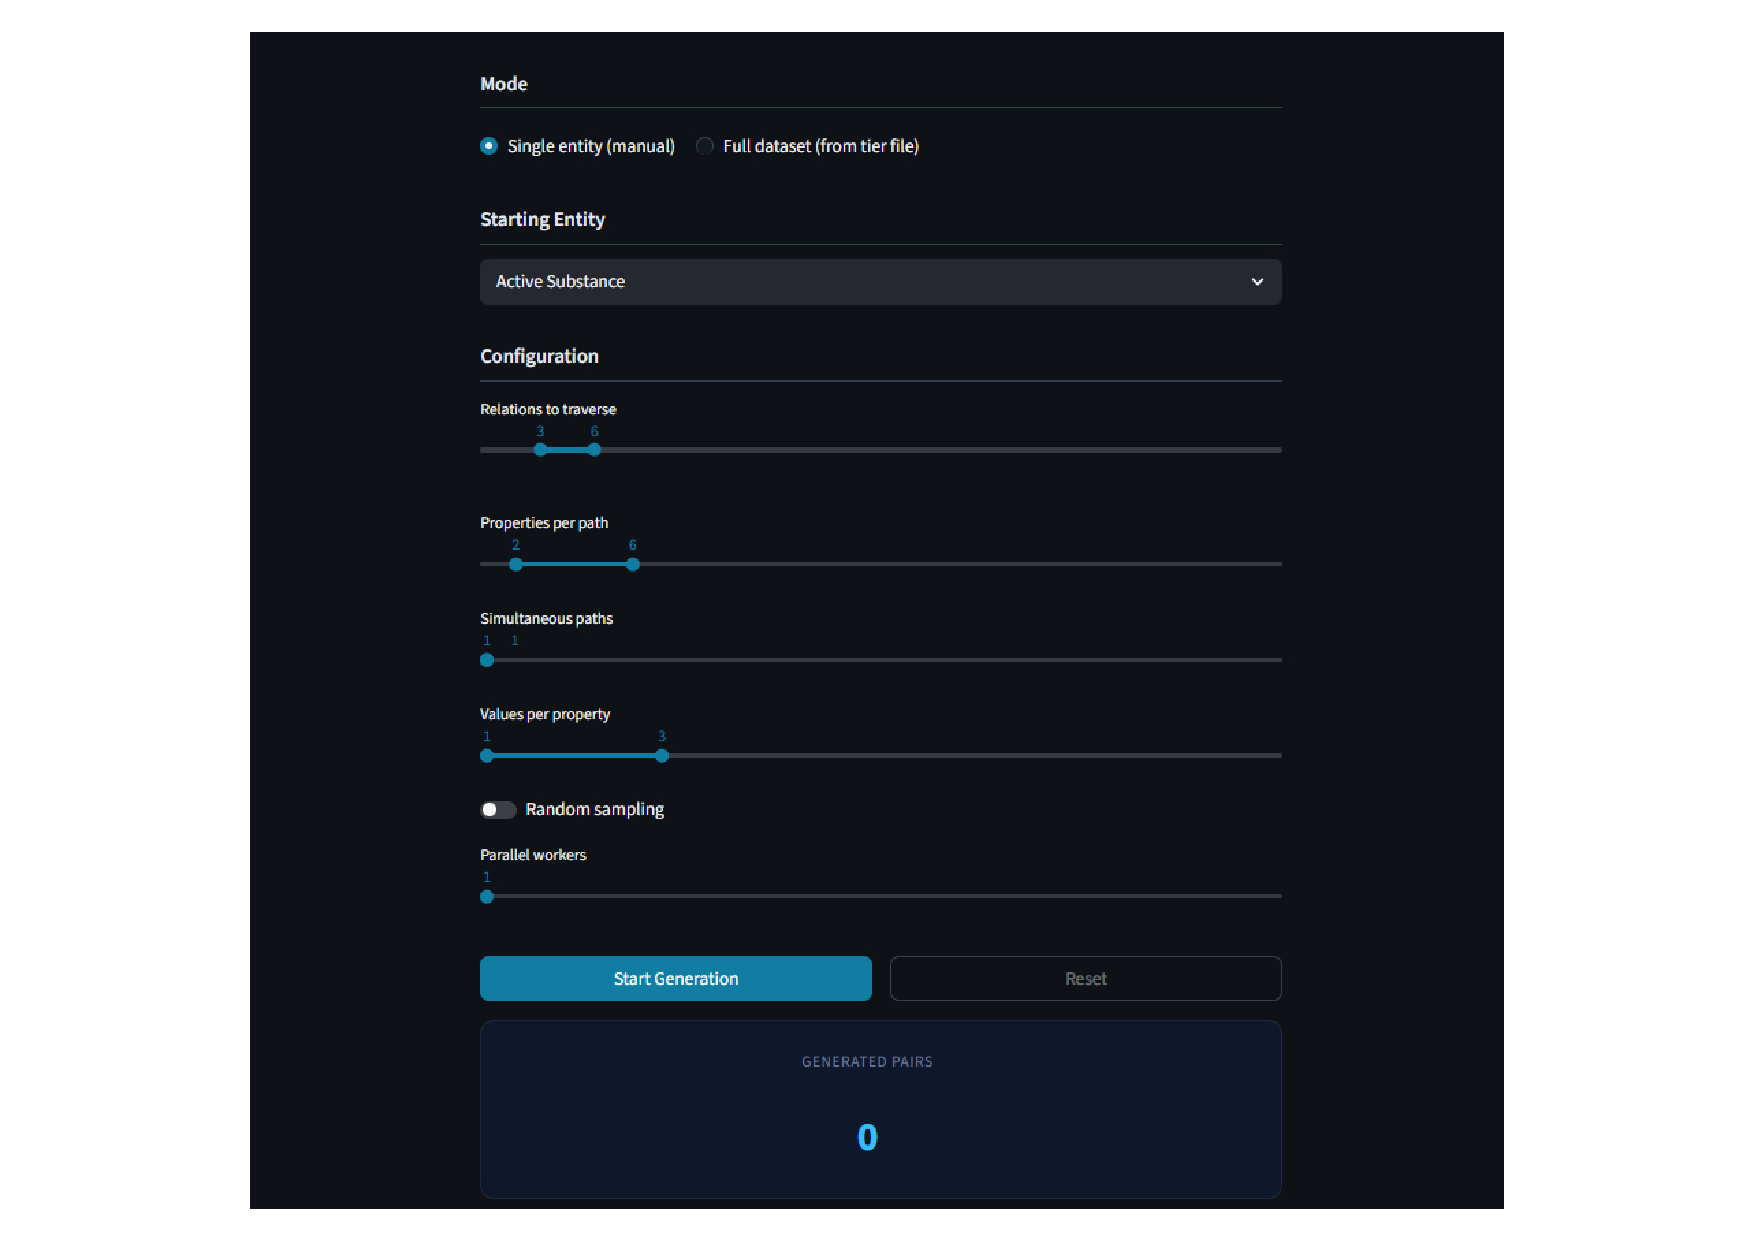
\includegraphics[width=1\linewidth]{figures/manual-generation-mockup.pdf}
%    \caption{Panoramica dell'interfaccia di controllo e calibrazione sviluppata
%    in Streamlit per la generazione interattiva su singola entità. La figura
%    illustra la sezione di selezione dell'entità radice e i quattro controlli
%    parametrici adibiti alla modulazione della complessità, evidenziando il
%    riscontro visivo dinamico sulle route effettivamente scoperte nel grafo.
%    Per brevità di rappresentazione, le sezioni relative alle modalità di
%    esecuzione e di gestione dello storico sono omesse, trovando già
%    dettagliata trattazione nel testo.} \label{fig:manual-mockup} \end{figure}

Questa modalità non è pensata per costruire un dataset completo, ma per
esplorare e calibrare. Al termine della generazione, infatti, il pannello non si
limita a riportare un conteggio finale, ma mostra due schede separate:
\begin{itemize}
    \item una con i record effettivamente creati, in un'anteprima tabellare di
          prompt e query
    \item una con quelli scartati, raggruppati per motivo di scarto esatto (tra
          cui i tre già discussi in \cref{sec:impl-output}) con la possibilità
          di filtrare e ispezionare i singoli tentativi falliti per una singola
          categoria
\end{itemize}

È proprio questo riscontro dettagliato a rendere la modalità manuale utile a
decidere quali parametri applicare a un tier con decine di entità e tempi di
generazione elevati, dove un errore nei parametri rischierebbe di sprecare
risorse di calcolo e prolungare inutilmente i tempi di attesa.

\subsection{Configurazione dei tier da file esterno}
\label{sec:impl-tier-config}

La modalità interattiva descritta nella sezione precedente consente
l'esplorazione di una singola entità alla volta; tuttavia, le diverse classi
dello schema richiedono parametri di generazione differenziati in base alla loro
rilevanza clinica, alla densità delle loro connessioni nel grafo e al volume di
varianti da rappresentare.

Per gestire questa eterogeneità, il generatore supporta la definizione di file
di configurazione esterni in cui le entità vengono raggruppate in insiemi
omogenei di parametri, denominati \emph{tier}. Tale astrazione evita
l'applicazione di vincoli uniformi all'intero schema o di ripetitive generazioni
manuali e permette di rendere le configurazioni riutilizzabili, tracciabili e
facilmente modificabili. Per ogni entità appartenente a un tier, il motore
\texttt{BulkDatasetGenerator} viene invocato applicando le impostazioni
specifiche di quel gruppo e un limite massimo di campioni per entità
(\texttt{sample\_size\_per\_entity}). I record generati dalle singole entità
vengono infine aggregati in un unico dataset primario per il successivo processo
di suddivisione (\cref{sec:impl-split}).

Nell'interfaccia Streamlit, la gestione dei tier è affidata a un modulo dedicato
che consente il caricamento del file di configurazione, la verifica preventiva
dei gruppi e il monitoraggio dell'avanzamento basato sul numero di entità
elaborate. Al termine del processo, il sistema rende disponibile il dataset
direttamente per il download, eliminando la necessità di accedere al filesystem
del server ospitante.

Infine, per garantire la robustezza dell'esecuzione, la configurazione dei tier
viene sottoposta a una procedura di validazione preventiva. Questa verifica
accerta la presenza delle chiavi obbligatorie, la validità dei range parametrici
e l'unicità dei nomi dei gruppi; un file non conforme viene rigettato all'atto
del caricamento con un'indicazione puntuale dell'errore, prevenendo interruzioni
anomale nelle fasi avanzate della generazione.

\begin{lstlisting}[language=Python, caption={Esempio minimo di configurazione di un tier da file JSON esterno.}, label={lst:tier-example}]
[ { "name": "diagnosis_related", "entities": ["Diagnosis", "TNMClassification"],
  "sample_size_per_entity": 50, "min_relations": 1, "max_relations": 3,
  "min_paths": 1, "max_paths": 2, "min_properties": 1, "max_properties": 3,
  "min_values": 1, "max_values": 2 } ]
\end{lstlisting}

\subsection{Split del dataset}
\label{sec:impl-split}

Una volta che tutte le entità dei tier configurati sono state processate e unite
in un unico file, l'ultimo passo divide i record in train, validation e test.

\begin{lstlisting}[language=Python, caption={Suddivisione del dataset in train, validation e test, stratificata per entità di origine.}, label={lst:split}]
for entity, recs in by_entity.items(): rng.shuffle(recs) n = len(recs) n_val =
    max(1, round(n * SPLIT_RATIOS["val"])) if n >= 10 else 0 n_test = max(1,
    round(n * SPLIT_RATIOS["test"])) if n >= 10 else 0 n_train = n - n_val -
    n_test splits["train"].extend(recs[:n_train])
    splits["val"].extend(recs[n_train:n_train + n_val])
    splits["test"].extend(recs[n_train + n_val:])
\end{lstlisting}

I record vengono raggruppati per entità di origine e suddivisi separatamente per
ciascun gruppo, con proporzioni 80/10/10 e seme fisso a 42 per la
riproducibilità (\cref{lst:split}), garantendo così che ogni entità sia
rappresentata nella stessa proporzione in tutti e tre gli split, invece di
rischiare che un'entità poco frequente finisca per puro caso quasi interamente
in uno solo di essi. Le entità con meno di 10 record totali non vengono
suddivise e finiscono interamente in train, perché un campione così piccolo non
permetterebbe una validazione o un test statisticamente significativi.

Lo split avviene prima dello stadio di augmentation, non dopo, per una ragione
precisa. Se l'augmentation venisse eseguita sull'intero dataset ancora unito,
più varianti parafrasate dello stesso record sorgente potrebbero finire sparse
su split diversi, contaminando la separazione tra train e test con esempi troppo
simili tra loro. Il generatore lo ricorda esplicitamente in un messaggio di log
al termine dello split, indicando di eseguire la pipeline di augmentation
separatamente su ciascuno dei tre file prodotti.

\section{Implementazione dell'augmentation}
\label{sec:impl-augmentation}

La fase di \textit{data augmentation} ha lo scopo di estendere la varietà
linguistica dei prompt generati dal primo stadio della pipeline, garantendo al
contempo che il significato semantico e i riferimenti puntuali alla query SPARQL
sottostante rimangano inalterati (\hyperref[obj:O2]{O2},
\hyperref[rnf:RNF3]{RNF3}).

Nelle prime fasi di esplorazione del progetto, la variazione stilistica è stata
affidata direttamente a un modello linguistico, fornendo il testo in chiaro e
richiedendone la rielaborazione in diversi registri linguistici (dallo stile
clinico-formale a quello colloquiale). Per questo compito di generazione è stato
impiegato il modello
\texttt{Gemma4:e2B}\footnote{\url{[https://ai.google.dev/gemma](https://ai.google.dev/gemma)}},
eseguito in locale tramite il runtime di inferenza
Ollama\footnote{\url{https://ollama.com}}, selezionato in quanto rappresentativo
di un ottimo compromesso tra qualità della riformulazione testuale, ridotto
ingombro computazionale e celerità di inferenza nell'esecuzione locale.

Tuttavia, l'affidamento diretto al modello senza vincoli strutturali si è
scontrato con i limiti pratici derivanti dall'impiego di un'architettura locale
di taglia contenuta (\hyperref[vinc:V3]{V3}), vincolo imposto dalla necessità di
garantire il trattamento riservato dei dati sanitari su infrastruttura locale
(\hyperref[vinc:V2]{V2}):

\begin{enumerate}
    \item \textbf{Alterazione e perdita di valori clinici
              (\textit{hallucination}):} Sebbene capace di buona fluidità
          sintattica, il modello locale tendeva a modificare o omettere
          identificativi, date, codici clinici e valori booleani,
          compromettendo la corrispondenza univoca tra il prompt e i filtri
          della query SPARQL.
    \item \textbf{Instabilità al crescere della complessità:} All'aumentare del
          numero di vincoli e valori presenti nella domanda originale, la
          capacità del modello di conservare l'intero contesto degradava,
          portando all'omissione involontaria di intere clausole.
    \item \textbf{Convergenza stilistica:} Lasciato libero di rielaborare il
          testo senza una guida rigida, il modello tendeva a riproporre le
          medesime strutture sintattiche e aperture di frase ricorrenti,
          vanificando l'obiettivo di varietà stilistica.
\end{enumerate}

Per superare queste criticità e garantire un tasso di accettazione dei record
economicamente sostenibile (\hyperref[rnf:RNF1]{RNF1}), la pipeline di
augmentation è stata completamente riprogettata attorno a un meccanismo rigoroso
di \textbf{mascheramento dei valori letterali} (mediante placeholder opachi)
associato a un ciclo iterativo di \textbf{generazione guidata, validazione e
    fallback}.

Nelle sottosezioni seguenti vengono descritte le componenti software che
realizzano tale architettura.

\subsection{Mascheramento}
\label{sec:impl-mask}

\subsection{Mascheramento deterministico dei valori}
\label{sec:impl-masking}

Per isolare la struttura sintattica del prompt dai dati puntuali, la prima fase
della pipeline di \textit{augmentation} sostituisce ogni valore letterale con un
identificativo opaco del tipo \texttt{[VAL\_XXXX]}, dove \texttt{[XXXX]}, ovvero
la componente alfanumerica, viene generata dinamicamente (\cref{lst:mask}).

L'alfabeto impiegato per la creazione dei token (\texttt{TOKEN\_ALPHABET})
esclude deliberatamente i caratteri ambigui (\texttt{I}, \texttt{L}, \texttt{O},
\texttt{0}, \texttt{1}). Questa scelta nasce da un'evidenza emersa nelle prime
fasi di test, i modelli di lingua di piccole dimensioni mostravano un'elevata
frequenza di allucinazione e sostituzione indebita su certi caratteri,
probabilmente a causa della loro somiglianza visiva nei vettori di embedding. I
placeholder vengono generati all'interno di un insieme (\texttt{set}) per
garantire l'assoluta unicità dei token all'interno dello stesso record.

La funzione \texttt{mask} applica le sostituzioni basandosi direttamente sugli
intervalli posizionali (\textit{spans}) calcolati dal generatore
(\cref{sec:impl-phrasing}), evitando costose ed errate ricerche per sottostringa
a posteriori. Infine, per la gestione dei placeholder vengono impiegate due
espressioni regolari con scopi distinti:
\begin{itemize}
    \item \textbf{Versione rigorosa (\texttt{VAL\_RE}):} Riconosce
          esclusivamente la struttura esatta dei token generati, utilizzata per
          estrarre e ricomporre i valori autentici;
    \item \textbf{Versione permissiva (\texttt{LOOSE\_VAL\_RE}):} Rileva
          varianti sintatticamente storpiate o generate arbitrariamente,
          impiegata nella successiva fase di validazione per intercettare ed
          eliminare le allucinazioni del modello (\cref{sec:impl-validation}).
\end{itemize}

\begin{lstlisting}[
    language=Python,
    caption={Generazione dei placeholder escludendo i caratteri ad alta frequenza di allucinazione e mascheramento basato su posizioni.},
    label={lst:mask}
]
TOKEN_ALPHABET = "ABCDEFGHJKMNPQRSTUVWXYZ23456789"

def generate_placeholder_tokens(n):
    tokens = set()
    while len(tokens) < n:
        token = "[VAL_" + "".join(random.choices(TOKEN_ALPHABET, k=4)) + "]"
        tokens.add(token)
    return list(tokens)

def mask(text, spans):
    spans = sorted(spans)
    tokens = generate_placeholder_tokens(len(spans))
    mapping, pieces, cursor = {}, [], 0
    
    for (start, end), placeholder in zip(spans, tokens):
        pieces.append(text[cursor:start])
        mapping[placeholder] = text[start:end]
        pieces.append(placeholder)
        cursor = end
        
    pieces.append(text[cursor:])
    return "".join(pieces), mapping
\end{lstlisting}

\subsection{Semplificazione booleana e generazione degli hint}
\label{sec:impl-boolean-hints}

Come anticipato nella fase di design, non tutti i placeholder mascherati
richiedono l'elaborazione da parte del modello linguistico. I valori booleani
vengono intercettati ed eliminati prima della fase di inferenza tramite la
funzione \texttt{simplify\_boolean\_phrasing} (\cref{lst:boolean}).

\begin{lstlisting}[
    language=Python,
    caption={Trascrizione proposizionale ed eliminazione preventiva dei placeholder booleani.},
    label={lst:boolean}
]
def simplify_boolean_phrasing(text, mapping):
    new_mapping = dict(mapping)
    for placeholder, value in mapping.items():
        if value.lower() not in {"true", "false"}:
            continue
            
        is_true = value.lower() == "true"
        repl = r"with \1" if is_true else r"without \1"
        esc = re.escape(placeholder)
        stop = r"(?:with|which|and)"
        
        which_re = re.compile(
            rf"\bwhich ((?:(?!{stop}\b)\w+ ?){{1,5}}) is {esc}", 
            re.IGNORECASE
        )
        with_re = re.compile(
            rf"\bwith ((?:(?!{stop}\b)\w+ ?){{1,5}}) {esc}", 
            re.IGNORECASE
        )
        
        if which_re.search(text):
            text = which_re.sub(repl, text)
            del new_mapping[placeholder]
        elif with_re.search(text):
            text = with_re.sub(repl, text)
            del new_mapping[placeholder]
            
    return text, new_mapping
\end{lstlisting}

La procedura analizza la struttura sintattica che circonda il token: un valore
booleano affermativo (\texttt{true}) viene convertito nella preposizione
\emph{"with"} seguita dal termine clinico di riferimento, mentre un valore
negativo (\texttt{false}) viene convertito in \emph{"without"}. L'operazione
rimuove il token sia dal testo sia dal dizionario di mappatura
(\texttt{new\_mapping}), sollevando le fasi successive della pipeline dalla
necessità di tracciare o ripristinare il valore.

Per tutti i restanti valori mascherati non booleani, il modulo invoca la
funzione \texttt{build\_hint\_map}, la quale costruisce un suggerimento in
linguaggio naturale (\textit{hint}) seguendo una gerarchia di regole
deterministiche ad alta priorità:

\begin{itemize}
    \item \textbf{Date in formato ISO:} Espresse in forma testuale estesa per
          preservare la naturalezza della frase;
    \item \textbf{Valori numerici interi ($< 1000$):} Convertiti dalla notazione
          cifrata alla corrispettiva forma letterale;
    \item \textbf{Etichette composte da trattino:} Semplificate isolando la
          componente terminologica specifica;
    \item \textbf{Fallback su modello linguistico:} Qualora nessuna delle
          trasformazioni euristiche sopra descritte sia applicabile, viene
          eseguita un'interrogazione mirata al modello per estrarre un sinonimo
          di uso comune nel dominio.
\end{itemize}

Il suggerimento così generato viene applicato, con una probabilità
configurabile, sia durante la fase di de-mascheramento e validazione finale
(\cref{sec:impl-validation}), sia come guida contestuale nella modalità di
generazione priva di mascheramento (\cref{sec:impl-nomask}).

\subsection{Suddivisione in chunk per record complessi}
\label{sec:impl-chunk}

All'aumentare della densità di placeholder in un singolo prompt, le prestazioni
del modello linguistico degradano visibilmente, portando a omissioni o alla
mancata rielaborazione di intere clausole. Per mitigare questo fenomeno, i
record con un numero elevato di valori mascherati vengono suddivisi in più
porzioni indipendenti (\textit{chunk}) prima di essere inoltrati al modulo di
generazione (\cref{lst:chunk}).

\begin{lstlisting}[
    language=Python,
    caption={Suddivisione in chunk del testo mascherato },
    label={lst:chunk}
]
MAX_VALUES_PER_CHUNK = 12

def split_into_chunks(masked_text, mapping, max_values_per_chunk):
    clauses = _protect_between(masked_text).split(CLAUSE_SEP)
    chunks = [[]]
    count_in_chunk = 0
    
    for clause in clauses:
        n_values = len(VAL_RE.findall(clause))
        if count_in_chunk > 0 and count_in_chunk + n_values > max_values_per_chunk:
            chunks.append([])
            count_in_chunk = 0
        chunks[-1].append(clause)
        count_in_chunk += n_values
        
    return [_restore_between(CLAUSE_SEP.join(c)) for c in chunks if c]
\end{lstlisting}

L'algoritmo segmenta il testo basandosi sulle congiunzioni coordinanti
(\emph{"and"}), aggregando le clausole in un unico chunk fino al raggiungimento
della soglia massima di 12 token (\texttt{MAX\_VALUES\_PER\_CHUNK}). Per evitare
la frammentazione incoerente di costrutti sintattici indivisibili, le funzioni
\texttt{\_protect\_between} e \texttt{\_restore\_between} mascherano
temporaneamente i connettivi interni alle espressioni di intervallo
(\emph{"between X and Y"}) sostituendoli con un carattere di controllo
esadecimale (NUL, \texttt{ASCII 0x00}).

I record il cui conteggio di valori rientra nella soglia limite non subiscono
alcuna suddivisione. A titolo esemplificativo, nella produzione del dataset da
1\,331 record generato con vincolo a 4 proprietà (\cref{sec:impl-tier-config}):
\begin{itemize}
    \item l'\textbf{80,6\%} dei casi (1\,073 record) ha prodotto un singolo
          chunk;
    \item il restante \textbf{19,4\%} (258 record) è stato ripartito esattamente
          su due chunk;
    \item nessun record ha necessitato di una frammentazione superiore a due
          chunk, con un caso limite di 20 token totali suddivisi in due
          sotto-porzioni rispettivamente da 11 e 9 valori.
\end{itemize}

\subsection{Ingegneria dei prompt e direttive di riformulazione}
\label{sec:impl-prompts}

La qualità e la robustezza delle parafrasi prodotte da \texttt{Gemma4:e2B}
dipendono in modo cruciale dalla struttura dei template di prompt inoltrati al
modello. Per guidare la generazione garantendo al contempo l'invarianza
semantica e sintattica, sono stati progettati tre template principali
(\cref{lst:prompt-templates}):

\begin{itemize}
    \item \textbf{\texttt{PROMPT\_TEMPLATE}:} Utilizzato per la rielaborazione
          completa dei prompt mascherati o del primo chunk. Definisce le regole
          tassative per la conservazione letterale dei token
          \texttt{[VAL\_XXXX]}, impone lo stile obiettivo, forza l'eliminazione
          delle ridondanze tipiche dei template rigidi (es. la semplificazione
          delle catene di navigazione relazionale del grafo) e vieta prefissi o
          metatesto nell'output.
    \item \textbf{\texttt{FRAG\-MENT\_\-\texttt{TEM\-PLATE}}:} Impiegato per i
          chunk successivi al primo (\texttt{as\_fra\-gment=True}). Omette le
          direttive stilistiche globali per mantenere il registro già stabilito,
          vieta la punteggiatura finale e impedisce l'inserimento della
          congiunzione coordinante iniziale (\emph{"and"}), affidandone la
          gestione al modulo di ricomposizione.
    \item \textbf{\texttt{NO\_MASK\_TEMPLATE}:} Utilizzato nella modalità di
          generazione priva di mascheramento dei valori
          (\cref{sec:impl-nomask}), in cui i valori letterali vengono forniti in
          chiaro affiancati da suggerimenti stilistici facoltativi
          (\textit{value hints}).
\end{itemize}

\begin{lstlisting}[
    language=Python,
    caption={Struttura dei template di prompt e funzioni per l'iniezione dinamica del contesto di feedback e storico.},
    label={lst:prompt-templates}
]
PROMPT_TEMPLATE = """Rewrite the following query request as a single reformulation in {language}.

Rules:
- The text below contains placeholders in square brackets, each one unique: copy each one EXACTLY as it appears, character-for-character.
- Every single placeholder in the original MUST appear, unchanged, in the reformulation.
- The original has a rigid template style: REMOVE repetition and phrase naturally.
- Compress awkward navigation chains (e.g. "which has height with metric unit [VAL]") into natural outcomes ("with a height measured in [VAL]") when intermediate steps add no value.
- Write it as {style}.
- Actively vary fact ordering: do not always follow the original traversal order.
{avoid_history_section}- Keep all clinical meaning exactly intact.
- Output ONLY the reformulation, nothing else.
{avoid_section}
Original: {question}

Reformulation:"""

def build_avoid_history_section(previous_texts: list) -> str:
    if not previous_texts:
        return ""
    items = "\n".join(f'  - "{t}"' for t in previous_texts)
    return (
        "- Do NOT reuse the wording, structure, or vocabulary of these previous "
        f"reformulations written in this same style:\n{items}\n"
    )

def build_avoid_section(avoid_text: str, reason: str = None) -> str:
    if not avoid_text:
        return ""
    reason_line = f" Specifically, the problem was: {reason}." if reason else ""
    return (
        f"\nA previous attempt was rejected.{reason_line} Do NOT repeat this mistake, "
        f"and do NOT repeat this wording - write something meaningfully different:\n\"{avoid_text}\"\n"
    )
\end{lstlisting}

Come mostrato nelle funzioni di supporto \texttt{build\_avoid\_history\_section}
e \texttt{build\_avoid\_section}, il sistema arricchisce dinamicamente il prompt
di input:
\begin{enumerate}
    \item \textbf{Preventivo anti-convergenza:} Iniettando le strutture
          sintattiche recentemente generate per lo stesso stile
          (\texttt{avoid\_history}), costringendo il modello a esplorare
          percorsi sintattici alternativi.
    \item \textbf{Feedback reattivo negli errori:} Inserendo nel ciclo di retry
          il testo scartato e la motivazione esplicita fornita dal validatore
          (\texttt{avoid\_reason}), trasformando la validazione in un meccanismo
          di apprendimento in-context guidato.
\end{enumerate}

\subsection{Generazione iterativa: stile, retry e fallback}
\label{sec:impl-generation}

Sfruttando le strutture di prompt e le funzioni di iniezione del contesto
descritte nella sezione precedente (\cref{sec:impl-prompts}), ogni
sotto-porzione (\textit{chunk}) e ogni successiva variante completa vengono
elaborate mediante un ciclo di generazione adattivo. La funzione
\texttt{generate\_piece} (\cref{lst:generate-piece}) orchestra i tentativi di
inferenza combinando un campionario a temperatura variabile, l'iniezione
dinamica del feedback e un meccanismo di fallback di sicurezza.

\begin{lstlisting}[
    language=Python,
    caption={Ciclo di generazione e validazione iterativa per un singolo chunk con gestione del fallback.},
    label={lst:generate-piece}
]
def generate_piece(
    model, piece_text, piece_mapping, style_desc, max_attempts,
    base_temp, max_temp, avoid_history, indent, label,
    avoid_text=None, avoid_reason=None, as_fragment=False,
    language="English"
):
    total_elapsed = 0.0
    for attempt in range(max_attempts):
        temperature = temperature_for_attempt(
            attempt, max_attempts, base_temp, max_temp
        )
        
        candidate, elapsed = (
            paraphrase_fragment(
                model, piece_text, piece_mapping, temperature, 
                language, avoid_text, avoid_reason
            )
            if as_fragment else
            paraphrase_one(
                model, piece_text, piece_mapping, style_desc,
                temperature, language, avoid_text, avoid_reason,
                avoid_history if attempt == 0 else None
            )
        )
        
        total_elapsed += elapsed
        reason = validation_reason(candidate, piece_mapping, [])
        
        if reason is None:
            return candidate, total_elapsed, False
            
        avoid_text, avoid_reason = candidate, reason
        
    return piece_text, total_elapsed, True
\end{lstlisting}

L'esecuzione del ciclo di generazione si articola sulle seguenti logiche
operative:

\begin{itemize}
    \item \textbf{Campionamento adattivo e ciclo di feedback:} Per ciascun
          tentativo (fino a un massimo di \texttt{max\_attempts}, pari a 5 di
          default), la funzione \texttt{temperature\_for\_attempt} calcola una
          temperatura di inferenza cresciuta linearmente da \texttt{base\_temp}
          a \texttt{max\_temp}. Se il candidato prodotto viene respinto dal
          validatore (\texttt{validation\_reason}), le variabili
          \texttt{avoid\_text} e \texttt{avoid\_reason} registrano l'output
          errato e il relativo motivo; tali informazioni vengono automaticamente
          convertite da \texttt{build\_avoid\_section} ed iniettate nel prompt
          del tentativo successivo, costringendo il modello a esplorare lo
          spazio latente in direzioni alternative.

    \item \textbf{Differenziazione tra primo chunk e frammenti successivi:} La
          generazione applica una diversa strategia a seconda della posizione
          del chunk. Il primo pezzo viene inviato tramite
          \texttt{paraphrase\_one} utilizzando il \texttt{PROMPT\_TEMPLATE}
          completo, comprensivo della descrizione dello stile e della cronologia
          delle strutture da evitare (\texttt{avoid\_history}). I chunk
          successivi vengono invece elaborati tramite
          \texttt{paraphrase\_fragment} (\texttt{as\_fragment=True}), inoltrando
          il \texttt{FRAGMENT\_TEMPLATE}; questa versione ridotta omette le
          direttive stilistiche globali e impedisce l'inserimento di
          congiunzioni o punteggiatura finale, garantendo la continuità
          sintattica con il primo frammento.

    \item \textbf{Garantismo e fallback deterministico:} Qualora tutti i
          tentativi consentiti falliscano a causa del persistere di violazioni
          sintattiche o di allucinazioni sui token, il sistema evita di forzare
          un testo degradato o incompleto. La funzione restituisce il testo
          mascherato originale non modificato (\texttt{piece\_text}), impostando
          il flag di fallback su \texttt{True}. In questo modo, la pipeline
          garantisce la continuità dell'esecuzione senza introdurre errori nel
          dataset. \end{itemize}

I controlli effettuati all'interno di \texttt{generate\_piece} sono strettamente
focalizzati sulla validità strutturale dei singoli chunk (come l'integrità dei
token di mascheramento). I controlli globali, tra cui il calcolo della
similarità sintattica rispetto ad altre varianti e il ripristino finale dei
valori, vengono posticipati alla fase di ricomposizione e validazione
dell'intero record (\cref{sec:impl-validation}).

\subsection{Validazione: due funzioni per due modalità}
\label{sec:impl-validation}

La validazione di un candidato applica fino a tre criteri in sequenza
all'interno di un'unica funzione (\cref{lst:validation}), più un quarto
controllo esterno sulla ripetizione dell'apertura di frase.

\begin{lstlisting}[language=Python, caption={La funzione di validazione condivisa da chunk e varianti complete, con soglia di somiglianza adattiva.}, label={lst:validation}]
def validation_reason(candidate, mapping, accepted_so_far, max_similarity=None):
    missing = [p for p in mapping if p not in candidate] if missing: return
    f"you dropped the placeholder(s) {', '.join(missing)} - every single one
    must appear unchanged"

    malformed = sorted(set(m for m in LOOSE_VAL_RE.findall(candidate) if m not
    in mapping)) if malformed: return f"you wrote malformed or invented
    placeholder-like text: {', '.join(malformed)} - placeholders must be copied
    exactly, never altered"

    threshold = max_similarity if max_similarity is not None else
    similarity_threshold_for(candidate) for prev in accepted_so_far: ratio =
    difflib.SequenceMatcher(None, candidate.lower(), prev.lower()).ratio() if
    ratio >= threshold: return f"this wording is too similar
    ({ratio:.0%} match) to a variant already produced for this same request"
    return None
\end{lstlisting}

Si parla di soglia di somiglianza adattiva poichè il controllo di somiglianza
\texttt{difflib.SequenceMatcher}\footnote{\url{https://docs.python.org/3/library/difflib.html}},
della libreria standard, varia a seconda della lunghezza del testo:
\begin{itemize}
    \item più permissiva (fino al 97\%) per frasi brevi
    \item più severa (85\%) per frasi lunghe
\end{itemize}
Questa piccola differenziazione è stata valutata come necessaria durante
l'implementazione, altrimenti testi corti sarebbero quasi sempre stati scartati
come duplicati per mancanza di margine di variazione lessicale.

Per la modalità di generazione priva di mascheramento (\cref{sec:impl-nomask}),
il sistema adotta una funzione di validazione dedicata, caratterizzata da un
criterio di verifica dei valori più flessibile. In questo scenario, poiché il
modello linguistico opera direttamente sui dati in chiaro con la facoltà
esplicita di applicarvi varianti stilistiche, un valore letterale non viene
classificato come omesso qualora compaia nel testo sotto forma di suggerimento
naturale (\textit{value hint}) o come sinonimo plausibile, valutato mediante un
confronto \textit{case-insensitive}.

\subsection{Rotazione degli stili e memoria anti-ripetizione}
\label{sec:impl-styles}

La diversificazione stilistica tra le differenti varianti di uno stesso record è
gestita dalla classe \texttt{StyleTracker} (\cref{lst:style-tracker}), la quale
assegna i registri espressivi in sequenza ed esegue un tracciamento a finestra
scorrevole delle generazioni recenti.

\begin{lstlisting}[
    language=Python,
    caption={Assegnazione ciclica degli stili e tracciamento a finestra delle formulazioni e delle aperture recenti.},
    label={lst:style-tracker}
]
class StyleTracker:
    def __init__(
        self, styles=None, recent_size=3, max_chars=160, opener_window=12
    ):
        self._styles = styles if styles is not None else STYLES
        self._style_cycle = itertools.cycle(self._styles)
        self._recent_texts = {tag: [] for tag, _ in self._styles}
        self._opener_history = {tag: [] for tag, _ in self._styles}
        self._recent_size = recent_size
        self._max_chars = max_chars
        self._opener_window = opener_window

    def next_style(self):
        return next(self._style_cycle)

    def remember(self, style_tag, text):
        sanitized = VAL_RE.sub("...", text)
        preview = (
            sanitized if len(sanitized) <= self._max_chars
            else sanitized[:self._max_chars - 3] + "..."
        )
        
        bucket = self._recent_texts.setdefault(style_tag, [])
        bucket.append(preview)
        del bucket[:-self._recent_size]
        
        openers = self._opener_history.setdefault(style_tag, [])
        openers.append(opener(text))
        del openers[:-self._opener_window]
\end{lstlisting}

L'assegnazione dei dieci registri linguistici predefiniti (spazianti dal tono
tecnico-database a quello colloquiale o statistico) avviene deterministicamente
mediante iterazione circolare
(\texttt{itertools.cycle}\footnote{\url{https://docs.python.org/3/library/itertools.html\#itertools.cycle}}).
Tale scelta previene i sbilanciamenti propri di un campionamento casuale,
assicurando una distribuzione uniforme dei registri sull'intero dataset.

Il metodo \texttt{remember} viene invocato esclusivamente a seguito
dell'accettazione di una variante, aggiornando due strutture dati distinte per
ciascun registro:

\begin{itemize}
    \item \textbf{Storico delle formulazioni complete
              (\texttt{\_recent\_texts}):} Mantiene una finestra delle ultime 3
          frasi generate. I token di mascheramento vengono preventivamente
          sostituiti con un punto di sospensione (\texttt{"..."}) per
          impedire che gli identificativi opachi alterino la valutazione
          della similarità testuale.
    \item \textbf{Storico delle aperture sintattiche
              (\texttt{\_opener\_history}):} Conserva una finestra più estesa,
          pari alle ultime 12 sequenze di avvio (\textit{openers}).
          Trattandosi di un'informazione a minore entropia rispetto alla
          frase intera, richiede uno storico più ampio per intercettare e
          neutralizzare pattern di incipit ricorrenti.
\end{itemize}

Il disaccoppiamento dei due tracciamenti in dizionari separati consente di
applicare metriche di controllo e orizzonti temporali differenti, evitando
riduzioni o troncamenti artificiali della memoria del modello.

\subsection{Statistiche di qualità e resilienza}
\label{sec:impl-stats}

Al fine di monitorare la qualità del processo di sintesi e garantire un
confronto tra le generazioni, ciascuna esecuzione della pipeline accumula un
insieme di metriche strutturate. Tali contatori permettono di tracciare la resa
qualitativa delle varianti generate, distinguendo le formulazioni prodotte con
successo da quelle derivanti da un meccanismo di fallback o dai fallimenti
definitivi (\cref{lst:qa-stats}).

\begin{lstlisting}[
    language=Python,
    caption={Calcolo della resa complessiva del processo di generazione e serializzazione delle metriche di qualità.},
    label={lst:qa-stats}
]
def to_dict(self):
    slots_failed = len(self.failed_slots)
    yield_rate = (
        (1 - (slots_failed / self.total_slots)) 
        if self.total_slots else None
    )
    return {
        "total_slots": self.total_slots,
        "slots_failed": slots_failed,
        "yield_rate": yield_rate,
        "fallback_count": self.fallback_count,
        "style_attempts": dict(self.style_attempts),
        "style_accepted": dict(self.style_accepted),
        "failed_slots": self.failed_slots,
    }
\end{lstlisting}

Il monitoraggio delle prestazioni si basa su tre indicatori principali:

\begin{itemize}
    \item \textbf{Tasso di resa (\texttt{yield\_rate}):} Esprime la quota di
          varianti generate con successo rispetto al totale degli slot richiesti
          (\texttt{total\_slots}).
    \item \textbf{Conteggio dei fallback (\texttt{fallback\_count}):} Traccia le
          varianti valide in cui almeno un chunk non è stato rielaborato dal
          modello ed è stato ripristinato nella forma originale per garantire la
          correttezza del record.
    \item \textbf{Slot falliti (\texttt{failed\_slots}):} Registra le richieste
          di variante per le quali, al termine di tutti i tentativi di
          rigenerazione previsti, non è stato possibile produrre un testo
          conforme. Per ciascun fallimento, la struttura dati conserva il
          tracciamento dettagliato dei tentativi e le relative cause di rifiuto.
\end{itemize}

Per soddisfare i requisiti di tolleranza ai guasti (\hyperref[rnf:RNF2]{RNF2}),
le statistiche vengono serializzate su disco a seguito dell'elaborazione di ogni
singolo record, in questo modo, in caso di interruzione imprevista
dell'esecuzione, un eventuale riavvio della pipeline non azzera i contatori ma
riprende lo stato accumulato. Parallelamente, un meccanismo di ripresa
automatica analizza i dati già salvati, ricostruendo l'elenco degli
identificativi (\texttt{source\_id}) completati ed evitando la rielaborazione
ridondante dei record.

\subsection{La modalità senza mascheramento}
\label{sec:impl-nomask}

Come anticipato il sistema conserva, per ciascun record, anche un percorso di
generazione alternativo che sottopone il testo intero privo di mascheramento al
modello con i valori veri elencati esplicitamente, senza alcuna suddivisione in
chunk (\cref{lst:nomask}).

\begin{lstlisting}[
    language=Python,
    caption={Implementazione della modalità baseline senza mascheramento per il confronto sperimentale.},
    label={lst:nomask}
]
def generate_variant_no_mask(
    model, text, values, style_tag, style_desc,
    max_attempts, base_temp, max_temp, avoid_history,
    slot_label, avoid_text=None, avoid_reason=None,
    language="English", hints=None
):
    # Deliberately no chunking here: this mode exists to reproduce
    # the pre-masking, single-shot behavior for direct comparison,
    # not to be a second production path.
    hints = hints or {}
    identity_mapping = {v: v for v in values}
    value_list = ", ".join(f'"{v}"' for v in values)
    
    # ... ciclo di retry e formattazione del prompt ...
    
    reason = validation_reason_with_hints(
        candidate, values, hints, []
    )
\end{lstlisting}

Durante la produzione del dataset qusto tipo di generazione non è stata
utilizzata, rappresenta quindi non un secondo percorso di produzione, ma un
termine di paragone diretto per valutare il beneficio del mascheramento
(\cref{chap:evaluation}). L'evidenza raccolta durante un'esecuzione diagnostica
su questa modalità conferma empiricamente le scelte progettuali presentate nel
\cref{chap:progettazione}. Su un totale di 41 rifiuti registrati nel log di un
test condotto su due record, ben 36 casi (pari all'87,8\%) sono stati causati
dalla perdita o dall'alterazione dei valori letterali da parte del modello. Tale
criticità viene resa strutturalmente impossibile dall'approccio basato su
mascheramento, in quanto il modello non ha mai accesso ai valori reali durante
la fase di riformulazione.

\chapter{Valutazione}
\label{chap:evaluation}

\section{Testing}
\label{sec:eval-testing}

\subsubsection{Problemi di qualità riscontrati e diagnosi delle cause}
\label{sec:eval-quality-issues}

Nel corso dello sviluppo e delle fasi di testing sono stati individuati e
analizzati cinque problemi di qualità principali (\cref{fig:quality-issues}), di
cui le relative proposte di risoluzione sono discusse nel
\cref{chap:conclusion}.

\begin{enumerate}
    \item \label{prob:ecog} \textbf{Scambio di acronimi clinici:} In un singolo
          caso, il modello di generazione dei sinonimi ha sostituito l'acronimo
          \texttt{ECOG} (relativo alla scala di stato funzionale oncologico) con
          la stringa riferita all'esame di ecocardiogramma. L'errore deriva dai
          limiti del modello locale di piccole dimensioni, che ha associato i
          due termini, basandosi con tutta probabilità, esclusivamente sulla
          somiglianza visiva del nome.

    \item \label{prob:icd10} \textbf{Allucinazione dei nomi di patologia sui
              codici ICD-10:} In 47 record, un medesimo codice ICD-10 è stato
          tradotto in nomi di patologie errate ed incoerenti tra le diverse
          formulazioni. La causa era un bug nella regex del filtro di
          sicurezza dei sinonimi, il quale escludeva i valori nel formato
          \texttt{PREFIX:CODE} se il prefisso era alfabetico (come per lo
          standard SNOMED \footnote{\url{https://www.snomed.org/}}), ma non
          intercettava il prefisso \texttt{ICD-10} perché contenente cifre.
          Il filtro di parsing è stato corretto, correggendo però solo in
          modo parziale il bug in questione.

    \item \label{prob:syntax} \textbf{Formattazione rigida e non naturale:}
          Durante l'ispezione manuale dei set di validazione e test, si è
          riscontrata la presenza di frasi formulate come liste di chiavi-valore
          o vere e proprie query anziché testo fluido. Il problema non dipendeva
          dal modello linguistico, ma dalla struttura troppo rigida degli stili
          di frase scritti manualmente, che sono stati di conseguenza
          rielaborati.

    \item \label{prob:dates} \textbf{Mancanza di connettivo negli intervalli di
              date:} In 55 occorrenze, due valori di data adiacenti sono stati
          affiancati senza alcun separatore (es. \emph{"2020-01-01
              2021-01-01"}), generando stringhe ambigue. La causa era
          un'omissione nella procedura di assemblaggio del testo, che non
          prevedeva l'inserimento della congiunzione tra due campi di tipo
          data consecutivi; il generatore è stato aggiornato per inserirla
          automaticamente.

    \item \label{prob:nan} \textbf{Presenza del valore nullo \texttt{"nan"}:} In
          7 casi è stata rilevata la stringa letterale \texttt{"nan"} indicata
          come unità di misura. Il comportamento è una probabile conseguenza del
          mascheramento deterministico, che preserva integralmente le stringhe
          ricevute in input senza modificarle. Il difetto risiederebbe quindi
          nella presenza di dati mancanti non filtrati a monte nel dataset
          primario.
\end{enumerate}

\begin{figure}[H]
    \centering
    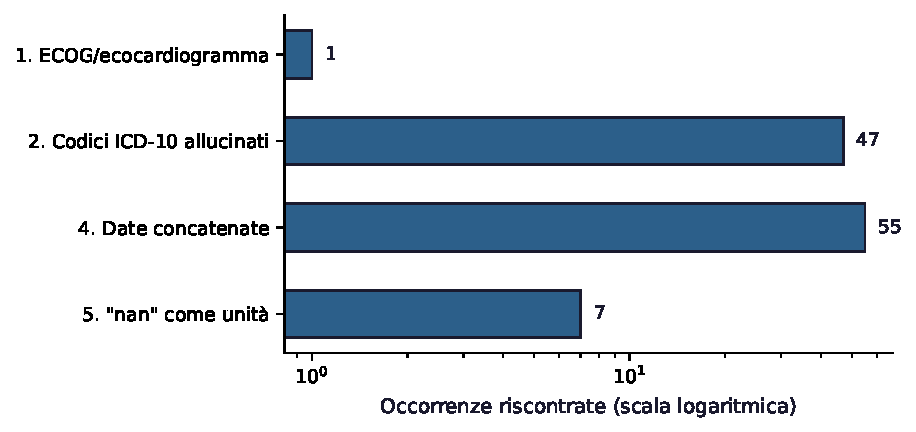
\includegraphics[width=.85\linewidth]{figures/quality-issues.pdf}
    \caption{Distribuzione delle occorrenze per i quattro problemi quantificabili (il problema di sintassi non naturale, individuato tramite ispezione manuale, non compare in figura).}
    \label{fig:quality-issues}
\end{figure}

\paragraph{Comportamenti anomali valutati come ammissibili.}
Due ulteriori fenomeni, inizialmente segnalati come bug, sono stati
ri-classificati come variazioni accettabili:
\begin{itemize}
    \item \textbf{Uso di preposizioni non canoniche (8 casi):} L'impiego di
          \emph{"at"} al posto di \emph{"on"} per le linee di terapia è stato
          considerato una naturale micro-variabilità del linguaggio umano, utile
          ad aumentare la varianza stilistica.
    \item \textbf{Collisione di vincoli incompatibili (295 casi):} La
          generazione di query con filtri reciprocamente escludenti (es. due
          date di decesso discordanti nella stessa query) deriva dal
          campionamento indipendente di percorsi relazionali paralleli. Poiché
          rispecchiano interrogazioni reali ma errate che un utente sbadato può
          porre, i record non costituiscono un difetto.
\end{itemize}

\subsubsection{Confronto tra generazione con e senza mascheramento}
\label{sec:eval-masking-comparison}

Per quantificare l'impatto del mascheramento sulla qualità della variazioni
stilistiche, è stato condotto un test comparativo rispetto alla modalità
no-masking, la cui architettura è stata documentata nella
\cref{sec:impl-nomask}. L'esperimento ha posto a confronto le due strategie su
un campione di 100 record sorgente, selezionati a complessità combinatoria
crescente (da un singolo valore vincolato fino a 20 valori simultanei per
query).

\begin{table}[H]
    \centering
    \small
    \renewcommand{\arraystretch}{1.2}
    \begin{tabularx}{\textwidth}{X c c}
        \toprule
        \textbf{Metrica / Criterio di Valutazione} & \textbf{Con Mascheramento}
                                                   & \textbf{Senza
                                                         Mascheramento}
        \\
        \midrule
        Slot di generazione totali                 & 330
                                                   & 330                             \\
        \textbf{Tasso di successo globale}         & \textbf{98,2\%} (324/330)
                                                   & \textbf{89,1\%} (294/330)
        \\
        Tasso di allucinazione sui valori          & \textbf{0,0\%} (0/330)
                                                   & \textbf{8,2\%} (27/330)
        \\
        Causa primaria di rigetto                  & Similarità parziale
        ($<90\%$)                                  & Duplicazione identica ($100\%$)
        \\
        Preservazione valori letterali             & Garantita per costruzione
                                                   & Modello-dipendente
        \\
        \bottomrule
    \end{tabularx}
    \caption{Confronto sperimentale tra la generazione con e senza mascheramento.}
    \label{tab:masking-comparison}
\end{table}

Come evidenziato nella \cref{tab:masking-comparison}, la valutazione su 330 slot
complessivi mostra un divario prestazionale netto a livello di tasso di
successo, in cui la modalità mascherata raggiunge raggiunge il \textbf{98,2\%},
contro l'\textbf{89,1\%} ottenuto dalla generazione senza mascheramento.

L'analisi dei log di scarto evidenzia due dinamiche qualitativamente differenti:
\begin{itemize}
    \item \textbf{Modalità senza mascheramento:} Il 10,9\% dei fallimenti totali
          è imputabile in massima parte (8,2\%) a violazioni dell'integrità dei
          dati (alterazione o omissione dei valori letterali) e in misura minore
          (2,7\%) a un collasso sintattico, in cui il modello ha rigenerato
          formulazioni identiche al 100\% a quelle già accettate.
    \item \textbf{Modalità con mascheramento:} I soli 6 rigetti registrati
          (1,8\%) sono derivati esclusivamente dal superamento della soglia di
          similarità adattiva su frasi brevi, senza alcuna corruzione dei token
          di mascheramento.
\end{itemize}

Questo comportamento è in gran parte riconducibile alle dimensioni contenute del
modello linguistico impiegato (\texttt{Gemma4:2B}). Infatti architetture locali
di piccola taglia, quando sollecitate a riformulare un testo mantenendo visibili
i dati in chiaro, faticano a disaccoppiare la struttura sintattica dal contenuto
informativo; di conseguenza, tendono a collassare su pattern espressivi rigidi o
ad allucinare le stringhe letterali. In questo modo abbiamo dimostrato che
l'introduzione dei placeholder opachi solleva il modello dal carico di memoria
sui dati, consentendogli di concentrare la capacità parametrica residuale
unicamente sulla variazione stilistica della frase.

\subsubsection{Statistiche del dataset}
\label{sec:eval-dataset-stats}

Il dataset finale risulta suddiviso in tre insiemi distinti, destinati
rispettivamente all'addestramento, alla validazione, e al test del modello.
L'insieme di addestramento comprende 9\,976 varianti, prodotte a partire da
3\,443 record sorgente distinti, con una media di 2,90 varianti per record. Gli
insiemi di validazione e di test comprendono rispettivamente 2\,022 e 2\,023
varianti, prodotte a partire da 428 record sorgente distinti ciascuno, con una
media di 4,72 e 4,73 varianti per record, contro un obiettivo fisso di cinque
varianti per record non sempre raggiunto per intero. Nessun record sorgente
risulta condiviso tra i tre insiemi: la verifica sull'insieme dei relativi
identificativi conferma una separazione completa, coerente con l'obiettivo di
una valutazione di reale generalizzazione anziché di semplice memorizzazione.

La distribuzione delle varianti tra i dieci registri stilistici nell'insieme di
addestramento risulta ragionevolmente uniforme, pur non perfettamente bilanciata
(\cref{fig:style-distribution}): lo stile più rappresentato,
\emph{technical\_sql}, compare in 1\,237 varianti, contro le 569 dello stile
meno rappresentato, \emph{generational}, un rapporto di circa 2,2 a 1 tra il più
e il meno frequente.

\begin{figure}[H]
    \centering
    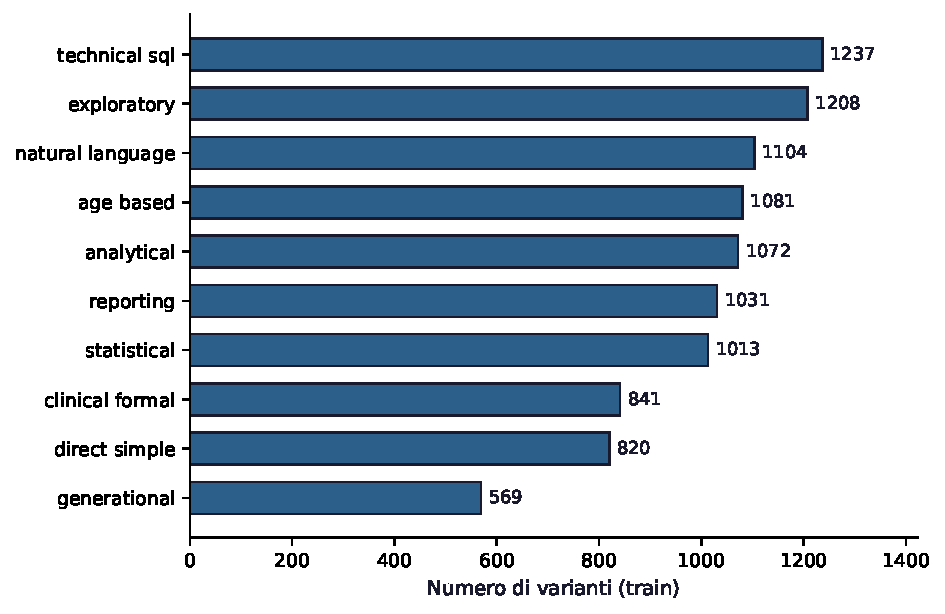
\includegraphics[width=.85\linewidth]{figures/style-distribution.pdf}
    \caption{Distribuzione delle varianti tra i dieci stili linguistici,
        nell'insieme di addestramento.}
    \label{fig:style-distribution}
\end{figure}

Una differenza rilevante nella densità di parafrasi si osserva tra l'insieme di
addestramento, prodotto tramite la formula adattiva basata sul numero di valori
per record, e gli insiemi di validazione e di test, prodotti con un numero fisso
di varianti per record: il primo presenta una media sensibilmente più bassa
(2,90 contro le circa 4,7 degli altri due insiemi), una scelta deliberata per
contenere il volume complessivo di addestramento senza sacrificare la varietà
stilistica degli insiemi usati per la misurazione delle prestazioni.

Infine, la quota di varianti non riformulate rispetto al testo originale
(\emph{fallback}) risulta contenuta in tutti e tre gli insiemi: 0,58\% nel train
(58 varianti su 9\,976), 0,35\% sia in validation sia in test (7 varianti
ciascuno).

\section{Experimental evaluation / demos}
\label{sec:eval-experimental}

Questa sezione riporta i risultati sperimentali del fine-tuning del modello
linguistico sul dataset descritto nella sezione precedente, confrontando diverse
configurazioni e analizzando la natura degli errori residui.

\subsubsection{Metodologia}

Il modello impiegato è \texttt{Gemma3:270M}, adattato tramite LoRA
(\cref{sec:peft-lora}) su un insieme di addestramento coerente con quello
descritto in \cref{sec:eval-dataset-stats}. La metrica principale è
l'\emph{exact match}, la percentuale di query generate identiche carattere per
carattere alla query di riferimento, calcolata su un insieme di test di cento
esempi in stile coerente con l'insieme di addestramento
(\emph{trainstyle-test}); dove indicato, i risultati sono riportati anche su un
secondo insieme di cento esempi fuori distribuzione (\emph{claude-test}),
formulato da un modello linguistico diverso da quello impiegato nella
generazione del dataset stesso, per verificare la capacità di generalizzazione a
formulazioni non viste in addestramento.

\subsubsection{Selezione del checkpoint}

Un primo addestramento di riferimento, condotto per 4\,000 iterazioni, è stato
seguito da un secondo addestramento più lungo, di 15\,000 iterazioni. Anziché
impiegare il checkpoint dell'ultima iterazione di quest'ultimo, la scelta è
ricaduta sul checkpoint con la \emph{validation loss} più bassa osservata
durante l'addestramento, in corrispondenza dell'iterazione 7\,000
(\cref{fig:loss-curve}). Questa scelta metodologica si è rivelata determinante,
portando l'exact match dal 15\% del checkpoint finale (iterazione 15\,000) al
46\% del checkpoint scelto, sullo stesso modello e sugli stessi dati di
addestramento.

\begin{figure}[H]
    \centering
    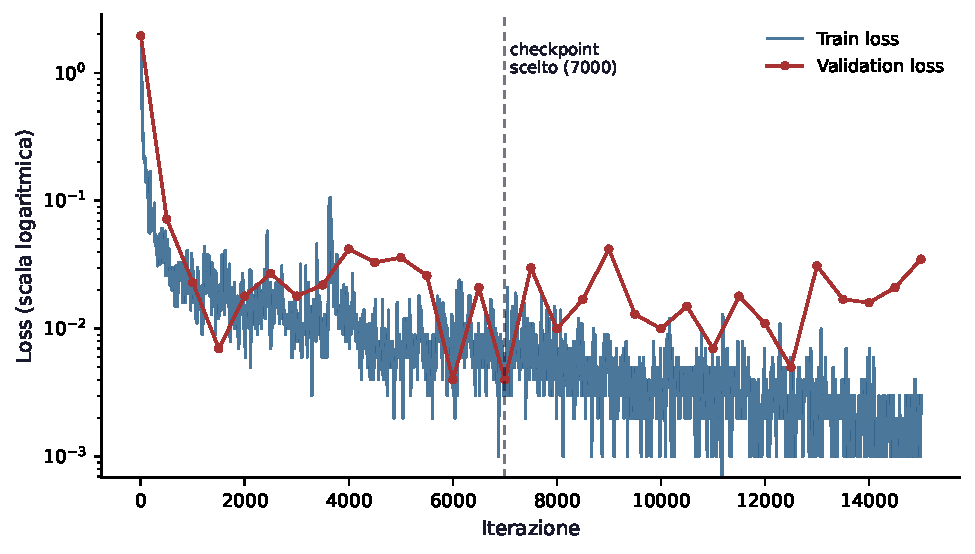
\includegraphics[width=.85\linewidth]{figures/loss-curve.pdf}
    \caption{Andamento della train e della validation loss durante
        l'addestramento di 15\,000 iterazioni. Il checkpoint scelto per la
        valutazione finale, in corrispondenza del minimo della validation loss,
        è evidenziato dalla linea tratteggiata.}
    \label{fig:loss-curve}
\end{figure}

\subsubsection{Confronto tra configurazioni}

Il checkpoint scelto (iterazione 7\,000) raggiunge un exact match del
\textbf{46\%} sull'insieme di test in stile coerente con l'addestramento, un
risultato solido per un modello di 270 milioni di parametri, addestrato con una
tecnica efficiente come LoRA, su un compito che richiede di produrre query
sintatticamente corrette e semanticamente vincolate a un'ontologia clinica reale
(\cref{fig:finetuning-comparison}). Il primo addestramento, più breve, aveva
raggiunto solo il 13\% nella stessa condizione, confermando che l'esposizione
prolungata ai dati, unita a una selezione accurata del checkpoint, produce un
miglioramento sostanziale e non marginale. Un confronto diretto con il full
fine-tuning, condotto sullo stesso modello di base per 6\,000 iterazioni, mostra
un exact match del 18\% nella medesima condizione, sensibilmente inferiore al
risultato ottenuto con LoRA a parità di ordine di grandezza di iterazioni.

\begin{figure}[H]
    \centering
    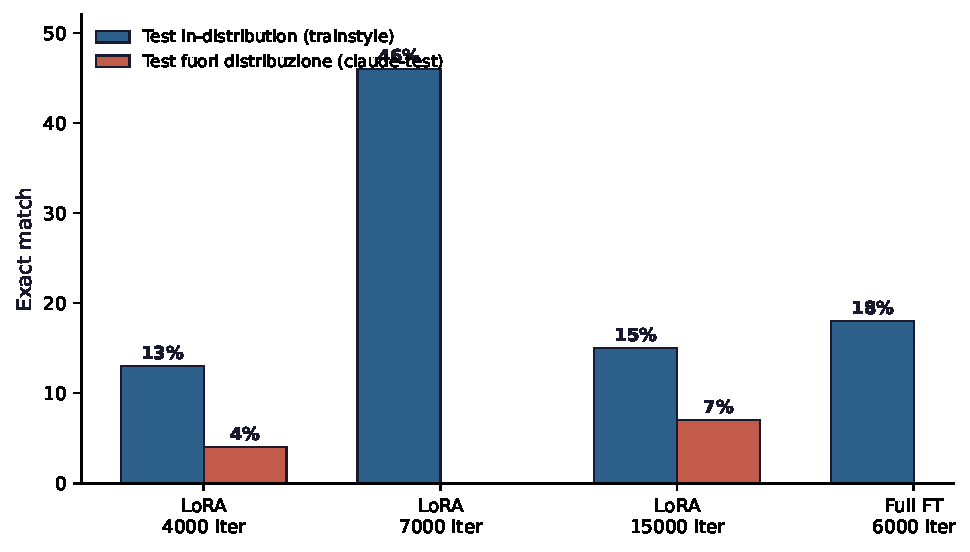
\includegraphics[width=.85\linewidth]{figures/finetuning-comparison.pdf}
    \caption{Confronto dell'exact match tra le configurazioni testate, sia
        sull'insieme di test in stile coerente con l'addestramento sia, dove
        disponibile, sull'insieme fuori distribuzione.}
    \label{fig:finetuning-comparison}
\end{figure}

Sull'insieme di test fuori distribuzione, i risultati sono naturalmente più
contenuti (4\% per il primo addestramento, 7\% per il checkpoint finale del
secondo), un calo atteso trattandosi di formulazioni mai osservate durante
l'addestramento e generate da un modello linguistico diverso da quello usato per
produrre il dataset. Il checkpoint scelto (iterazione 7\,000) non è stato
valutato su questo insieme, essendo stato individuato successivamente come il
più promettente sulla base della sola validation loss.

\subsubsection{Analisi degli errori}

Le cinquantaquattro righe non corrispondenti esattamente al checkpoint scelto
sono state analizzate confrontando in modo automatico la struttura e i valori di
ciascuna query generata con quella di riferimento (\cref{fig:error-taxonomy}).
Nella maggioranza dei casi, il 63\%, la query generata utilizza un predicato,
una classe, o un percorso relazionale diverso da quello corretto, tipicamente
confondendo entità ontologiche simili tra loro (ad esempio \texttt{Patient} con
una sua sottoclasse come \texttt{DrinkerPatient}, introdotta nella query senza
che il prompt la richiedesse). Nel 24\% dei casi la struttura della query è
corretta, ma uno dei valori letterali richiesti differisce da quello atteso. Nel
restante 13\% dei casi, la query è strutturalmente corretta e utilizza il
predicato giusto, ma restituisce un identificativo o un codice errato al posto
di quello corretto, ad esempio confondendo due codici della classificazione
ICD-10 entrambi plausibili nel contesto ma diversi da quello richiesto.

\begin{figure}[H]
    \centering
    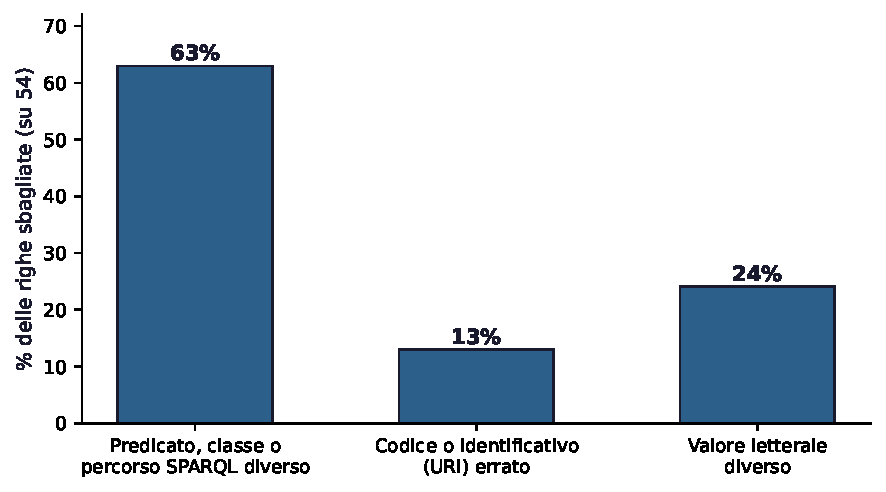
\includegraphics[width=.75\linewidth]{figures/error-taxonomy.pdf}
    \caption{Distribuzione delle cinquantaquattro righe non corrispondenti per
        categoria di errore, sul checkpoint scelto (iterazione 7\,000).}
    \label{fig:error-taxonomy}
\end{figure}

È significativo che, in nessuno dei casi analizzati, il modello abbia prodotto
una query non sintatticamente valida o strutturalmente incoerente. Anche negli
errori, il modello dimostra di aver appreso in modo affidabile la grammatica del
linguaggio di interrogazione e la struttura generale delle query attese,
concentrando le proprie difficoltà in un numero limitato di pattern
riconoscibili e riconducibili a una causa comune, la discriminazione tra entità
o valori simili tra loro, più che a un comportamento arbitrario o imprevedibile.

\chapter{Conclusioni e sviluppi futuri}
\label{chap:conclusion}

Questo lavoro ha affrontato il problema della mancanza di un dataset di
addestramento per un modello linguistico capace di tradurre domande in
linguaggio naturale in query SPARQL sul knowledge graph del Cancer Virtual Lab,
progettando e implementando una pipeline automatica in due stadi per costruirlo,
e verificandone l'efficacia tramite il fine-tuning concreto di un modello
linguistico sui dati prodotti.

I quattro obiettivi specifici definiti in \cref{chap:analisi} possono essere
considerati raggiunti. La \hyperref[obj:O1]{copertura selettiva ed
    estendibilità} (\textbf{O1}) è stata ottenuta tramite il meccanismo dei tier,
che copre quarantacinque entità dello schema senza richiederne la copertura
completa, ed è estendibile a nuove classi tramite una configurazione esterna che
non richiede di modificare il codice del generatore
(\cref{sec:impl-tier-config}). La \hyperref[obj:O2]{varietà linguistica
    autentica} (\textbf{O2}) è stata perseguita tramite lo stadio di augmentation,
che produce dieci registri stilistici distinti a partire da ciascuna coppia
generata, con un tasso di successo superiore al 97\% anche nella modalità più
restrittiva testata (\cref{sec:eval-masking-comparison}). La
\hyperref[obj:O3]{tracciabilità completa} (\textbf{O3}) è garantita
dall'identificativo di provenienza mantenuto per ogni variante, verificato non
presentare alcuna sovrapposizione tra gli insiemi di addestramento, validazione
e test (\cref{sec:eval-dataset-stats}). Il \hyperref[obj:O4]{volume di dati
    adeguato al fine-tuning} (\textbf{O4}) è confermato non solo dal numero
complessivo di quattordicimilaventuno varianti prodotte, ma soprattutto dal
fatto che il dataset si sia dimostrato concretamente utilizzabile per addestrare
un modello con risultati misurabili, come riportato di seguito.

La valutazione sperimentale del modello ottenuto tramite fine-tuning ha prodotto
un risultato solido, un exact match del 46\% su un insieme di test in stile
coerente con l'addestramento, ottenuto con LoRA su un modello di soli 270
milioni di parametri (\cref{sec:eval-experimental}). Due risultati metodologici
emersi durante la valutazione meritano di essere sottolineati. Il primo è che la
scelta del checkpoint in base alla validation loss, piuttosto che all'ultima
iterazione disponibile, ha prodotto un miglioramento determinante, dal 15\% al
46\% di exact match a parità di modello e di dati. Il secondo è che, a parità di
ordine di grandezza di iterazioni, LoRA ha superato nettamente il full
fine-tuning condotto come confronto (46\% contro 18\%). L'analisi degli errori
residui ha inoltre mostrato che nessuno di essi consiste in una query
sintatticamente non valida: il modello ha appreso in modo affidabile la
grammatica del linguaggio di interrogazione, concentrando le proprie difficoltà
nella discriminazione tra entità o valori simili tra loro, piuttosto che in un
comportamento arbitrario.

Il processo di sviluppo ha inoltre permesso di individuare e diagnosticare
cinque problemi di qualità genuini nel dataset generato
(\cref{sec:eval-quality-issues}), riconducendo ciascuno alla propria causa
tecnica; due di essi sono già stati corretti nell'ambito di questo lavoro,
mentre per i restanti tre è proposta una via di correzione nella sezione
seguente. Due ulteriori comportamenti, inizialmente considerati problematici,
sono stati infine riconosciuti come accettabili, un risultato che riflette una
comprensione più matura, maturata nel corso del lavoro, di cosa costituisca
realmente un difetto in un dataset di questo tipo rispetto a una variazione
legittima.

\section{Sviluppi futuri}
\label{sec:future-work}

\subsection{Risoluzione dei problemi di qualità}
\label{sec:future-quality-fixes}

Alcuni dei problemi di qualità discussi in \cref{sec:eval-quality-issues} non
hanno ricevuto, nell'ambito di questo lavoro, una correzione alla radice, e
rappresentano quindi possibili direzioni di sviluppo futuro.

\textbf{Confusione tra acronimi clinici simili}
(\cref{sec:eval-quality-issues}, p.~\pageref{prob:ecog}). Una possibile
correzione consisterebbe nel restringere la generazione di sinonimi per questa
categoria di valori a un dizionario curato di equivalenze verificate, invece di
affidarsi alla generazione libera del modello linguistico locale, che non
dispone di una base affidabile di terminologia clinica.

\textbf{Allucinazione di codici ICD-10}
(\cref{sec:eval-quality-issues}, p.~\pageref{prob:icd10}). Il difetto specifico
nel filtro di riconoscimento è già stato corretto, ma una correzione più robusta
consisterebbe nell'escludere del tutto dalla generazione libera qualunque valore
riconducibile a un sistema di codifica controllato, sostituendola con una
verifica rispetto alla tabella dei codici validi prima di accettare qualunque
sostituzione proposta, così da eliminare il rischio alla radice invece di
limitarsi a riconoscere meglio i pattern da escludere.

\textbf{Valore letterale "nan" come unità di misura}
(\cref{sec:eval-quality-issues}, p.~\pageref{prob:nan}). Una correzione
consisterebbe nel riconoscere esplicitamente questo tipo di valore mancante
durante la generazione del dataset strutturato, escludendo il record interessato
o rappresentando l'assenza del dato in modo esplicito, invece di lasciare che un
segnaposto tecnico non gestito raggiunga il testo finale.

\subsection{Altre direzioni di sviluppo}
\label{sec:future-other}

Oltre alla risoluzione dei problemi di qualità appena discussi, il lavoro
suggerisce alcune direzioni di sviluppo più ampie, emerse dai limiti riscontrati
nel corso della valutazione più che da difetti puntuali.

\textbf{Estensione della copertura dello schema}. Il dataset attuale copre
quarantacinque entità dello schema (\hyperref[obj:O1]{O1}), una scelta selettiva
e non esaustiva. Il meccanismo di configurazione dei tier tramite file esterno
(\cref{sec:impl-tier-config}) rende possibile estendere questa copertura ad
altre classi e relazioni del knowledge graph senza modificare il codice del
generatore; sfruttare concretamente questa possibilità per ampliare il dataset
resta un lavoro da svolgere.

\textbf{Valutazione a livello di esecuzione}. La metrica di valutazione
impiegata in questo lavoro, l'exact match, richiede una corrispondenza carattere
per carattere tra la query generata e quella di riferimento
(\cref{sec:eval-experimental}). Una query semanticamente equivalente ma
formulata in modo sintatticamente diverso, ad esempio con clausole in un ordine
differente, viene quindi conteggiata come errore anche quando produrrebbe lo
stesso risultato se eseguita sul knowledge graph. Una valutazione complementare,
che esegua le query generate sull'endpoint di CVL e ne confronti i risultati
restituiti anziché il solo testo, fornirebbe una stima più accurata delle
prestazioni reali del modello.

\textbf{Altre tecniche o modelli di adattamento}. Questo lavoro ha confrontato
LoRA con il full fine-tuning (\cref{sec:eval-experimental}), ma non ha testato
QLoRA, pure introdotta in \cref{sec:peft-lora} come tecnica in grado di ridurre
ulteriormente l'occupazione di memoria rispetto a LoRA; allo stesso modo, non
sono stati testati modelli di base diversi da \texttt{Gemma3:270M}, di
dimensioni maggiori o architettura differente, che potrebbero offrire una
migliore capacità di generalizzazione a scapito di un costo computazionale più
elevato.

\textbf{Resilienza a interruzioni estesa al generatore}. Il requisito di
resilienza a interruzioni (\hyperref[rnf:RNF2]{RNF2}) è soddisfatto dallo stadio
di augmentation, che ricostruisce a ogni avvio l'elenco dei record già
processati, ma non dal generatore, che non conserva alcuna informazione tra
un'esecuzione interrotta e la successiva. Estendere un meccanismo analogo anche
al generatore ridurrebbe il lavoro perso in caso di interruzione durante le fasi
iniziali della pipeline.

\backmatter


\bibliographystyle{alpha}
\bibliography{bibliography}

\end{document}